\documentclass{automatextcc}
\usepackage{ulem}
\usepackage{dsfont}
\usepackage{placeins}
%\usepackage{refcheck}
\usepackage{enumitem}

\usepackage[table]{xcolor}


\usepackage{booktabs}
\usepackage{multirow}

\usepackage{array}

% Caminho da Pasta das Figuras
\graphicspath{{figuras/}}

%\makeindex  Opcional (Índice Remissivo)

%\newcommand{\obs}[1]{\textcolor{purple}{#1}}
%\newcommand{\nico}[1]{\textcolor{teal}{#1}}
\newcommand{\pumi}[1]{\textcolor{red}{#1}}
\newcommand{\red}[1]{\textcolor{red}{#1}}
\newcommand{\blue}[1]{\textcolor{blue}{#1}}

\newcommand{\R}{\mathds{R}}
\newcommand{\N}{\mathds{N}}
\newcommand{\B}{\mathds{B}}
\newcommand{\Perp}{\mathcal{P}}
\newcommand{\bs}[1]{\boldsymbol{#1}}



\begin{document}


\title{Composição Automática de Músicas utilizando Redes Neurais Recorrentes}
\author{Nicolas Mathias Hahn}

% orientador(a) do trabalho {nome}{Orientador(a)}
\advisor{Prof. Dr. Guilherme Pumi}{Orientador}
% universidade onde obteve o título e atual
\advisorinfo{Doutor pela Universidade Federal do Rio Grande do Sul, Porto Alegre, RS}{UFRGS}

% banca examinadora:
\examinera{Prof. Dr. João Henrique Ferreira Flores}
\examinerainfo{Doutor pela Universidade Federal do Rio Grande do Sul, Porto Alegre, RS}{UFRGS}

% departamento:
\dept{\DEST}

% data de entrega:
\date{Outubro de 2022}


% Capa
\maketitulo

% Folha de rosto
\makefolhaderosto

% Folha de aprovação
\makefolhadeaprovacaoA % Um membro na banca
%\makefolhadeaprovacaoB % Dois membros na banca


% Epígrafe (OPCIONAL)
\newpage
\vspace*{\fill}
\begin{flushright} % mexer aqui
	\textit{``Since I have always preferred making plans to executing them, I have gravitated towards situations and systems that, once set into operation, could create music with little or no intervention on my part. That is to say, I tend towards the roles of planner and programmer, and then become an audience to the results.''} \newline
	\textit{Brian Eno \citep{alpern1995}}.
\end{flushright}

% Agradecimentos
%\newpage
%\chapter*{Agradecimentos}
%Agradeço a xxx. Opcional % mexer aqui

% palavras chave
    % português
\keyword{Música}
\keyword{Composição Musical}
\keyword{Redes Neurais Recorrentes}
\keyword{Processamento de Linguagem Natural}
    % inglês
\keyworde{Music}
\keyworde{Music Composition}
\keyworde{Recurrent Neural Networks}
\keyworde{Natural Language Processing}


% resumo 
    % português
\begin{abstract}
O problema de composição musical automática é extensivamente  explorado na literatura. Em geral, o objetivo final nesses trabalhos é a composição musical em si, de forma que os modelos utilizados são ajustados para que a música gerada seja adequada em algum sentido. Detalhes técnicos como os impactos que as modificações nos parâmetros tem na composição final, ainda, são amplamente desconhecidos. Neste trabalho, temos por objetivo estudar o quão sensível é um modelo de rede neural, baseado em processamento de linguagem natural, construído para composição musical. Para tal tarefa, a mensuração será feita com a perplexidade, uma medida oriunda da teoria da informação. Por fim, as músicas são avaliadas, de forma subjetiva, em relação à musicalidade e qualidade das peças musicais obtidas.
\end{abstract}

    % inglês
\begin{englishabstract}
The issue of automatically composed music has received a lot of attention in the literature. In general, the focus is on the composition itself, and models are tuned to produce useful results. Technical details such as the effects that adjustments to the model's parameters have on the composition, however, are still largely unknown. In this work, we investigate how sensitive is a neural network model, based on natural language processing,  built for music composition. To accomplish this task, we apply a metric from information theory called perplexity. The composed works are then subjectively assessed for musicality and quality.
\end{englishabstract}

% sumário (Obrigatório)
\tableofcontents

% lista de ilustrações (Obrigatório)
\listoffigures

% lista de tabelas (Obrigatório)
\listoftables



%%%%%%%%%%%%%%%%%%%%%%%%%%%%%%%%%%%
%%%%  Introdução
%%%%%%%%%%%%%%%%%%%%%%%%%%%%%%%%%%%
\chapter{Introdução}
Composição algorítmica, ou composição automática, refere-se ao processo de criação de músicas por meio de algum processo formal com pouca ou nenhuma intervenção humana. De acordo com \citet{maurer}, podemos encontrar três metodologias diferentes que existem em composição algorítmica: estocástica, \textit{rule-based} e inteligência artificial.

Wolfgang Amadeus Mozart (1756-1791) utilizou técnicas de composição algorítmica em sua obra \textit{Musikalisches Wurfelspiel} (\textit{Dice Music}), um jogo musical que envolvia atribuir um número para fragmentos de músicas, e combiná-los ao acaso, criando uma nova peça com as partes selecionadas. Além disso, John Cage (1912-1992), assim como Mozart, utilizou aleatoriedade em suas composições. Como exemplo, temos \textit{Reunion}, uma performance em que músicas são geradas ao jogar xadrez em um tabuleiro equipado com um foto receptor: cada lance emitia um som e, portanto, a música resultante é única por jogo. Por fim, com o auxílio de computadores, David Cope (1941-) criou, em 1981, o EMI (\textit{Experiments in Musical Intelligence}), um sistema baseado em grandes bases de dados com descrições de estilos de diferentes estratégias composicionais e, como complemento, o sistema também tinha a capacidade de criar as próprias regras composicionais por meio dos novos dados recebidos \citep{alpern1995, maurer}. 

Na literatura, encontramos diversos exemplos de trabalhos envolvendo composição musical automática. Os dados utilizados para o objetivo de composição podem vir tanto em formato de áudio \citep[como o de][]{kuang2021} quanto em formato de texto \citep[como o de][]{agarwala2017}. Ao mesmo tempo em que o trabalho de \citet{colombo2016} é claro em sua relação com a composição algorítmica, \citet{souza2018} é evasivo. Também, observou-se um foco em criação de músicas e avaliação das composições musicais, seja pela estrutura musical seja pela opinião de ouvintes referente à geração (se era musicalmente plausível). Por fim, os trabalhos de \citet{fernandez2013}, \citet{ji2020} e de \citet{olivan2021} são um sucinto resumo de abordagens e técnicas de inteligência artificial (como redes neurais artificiais) utilizadas para composição automática de músicas, assim como as formas de avaliação. 

O presente trabalho propõe-se a explorar o problema de composição algorítmica no contexto de modelagem, sendo as peças musicais geradas uma consequência dos modelos. Dessa forma, mesmo sem conhecimentos sobre teoria musical, é possível elencar um melhor modelo apenas por métricas objetivas. Por meio de técnicas de processamento de linguagem natural e de redes neurais artificiais, serão criados modelos capazes de composição com base em conjuntos de músicas na notação ABC. Devido a isso, os dados utilizados serão restritos ao formato textual. Dada a natureza subjetiva da música, as peças musicais resultantes serão subjetivamente avaliadas, comparando-as de acordo com a percepção do autor.



%%%%%%%%%%%%%%%%%%%%%%%%%%%%%%%%%%%
%%%%  Referencial Teórico
%%%%%%%%%%%%%%%%%%%%%%%%%%%%%%%%%%%
\chapter{Referencial Teórico}

% composição algorítmica
\section{Composição Algorítmica}
Composição algorítmica, ou composição automática, refere-se ao processo de criação de músicas por meio de algum processo formal com pouca ou nenhuma intervenção humana. O termo ``algoritmo'' é definido como um conjunto predeterminado de instruções com o objetivo de resolver um problema em específico com um número limitado de passos. O ``problema'' encarado por compositores é a composição musical, e as ``instruções'' predeterminadas sugerem que, uma vez que o processo é iniciado, a intervenção humana é substituída. Portanto, ``composição automática'' também descreve adequadamente esse tipo de composição musical, sendo que ``automático'' refere-se a ``qualquer coisa que pode se mover ou agir por conta própria'' \citep{alpern1995, maurer}.

De acordo com \citet{maurer}, podemos encontrar três metodologias diferentes que existem em composição algorítmica: 
\begin{itemize}
    \item \textbf{estocástica:} abordagem mais simples. Envolve aleatoriedade e pode ser tão simples quanto gerar uma série de notas musicais ao acaso, bem como sortear uma ordem de fragmentos de músicas para ser performada pelo músico.
    \item \textbf{\textit{rule-based}:} em vez de delegar decisões ao acaso como no método estocástico, um sistema \textit{rule-based} define uma ``constituição'' ou ``gramática'' (sistema formal de princípios ou regras que as possíveis frases de uma linguagem são geradas) em que o sistema deve seguir uma vez iniciado o processo de composição. 
    \item \textbf{inteligência artificial (IA): }similar ao ``rule-based'' no sentido de ser baseado em uma gramática pré-definida. No entanto, sistemas de IA têm a capacidade de definirem sua própria gramática, que pode evoluir (isto é, ser modificada de uma forma automática) ao longo do processo.
\end{itemize}
Mais detalhes podem ser encontrados em \citet{alpern1995}, \citet{maurer}, \citet{nierhaus2009}, \citet{fernandez2013} e \citet{olivan2021}.  



    % Redes Neurais Artificiais
\section{Redes Neurais Artificiais}
Redes Neurais Artificiais (RNA) são técnicas de aprendizagem de máquina inspiradas no mecanismo de aprendizagem presente em organismos vivos \citep{aggarwal2018}. Nos seus primórdios, os algoritmos tinham o intuito de ser um modelo computacional capaz de imitar a aprendizagem ocorrida no cérebro \citep{goodfellow2016}.



        % Redes Neurais e a Estatística
\subsection{Redes Neurais e a Estatística}
Muitos modelos de RNAs são similares ou idênticos a populares técnicas estatísticas como modelos lineares generalizados, regressão linear (simples e múltipla), regressão polinomial, regressão não paramétrica e análise discriminante (como a regressão logística), especialmente quando a ênfase é na predição de um fenômeno complexo em vez de sua explicação. Devido a esse foco em predição, RNAs são utilizadas como modelos \textbf{caixa preta}: uma certa entrada produz uma determinada saída da função, mas o processo interno que a rede utilizou para chegar nesse resultado é desconhecido e, consequentemente, há perda de interpretabilidade do modelo \citep{sarle1994, cheng1994, rojas1996}.

No contexto de RNAs, é possível definir dois procedimentos para a resolução de algum problema prático (aplicado): especificar a arquitetura da rede e treinar a rede com um conjunto de dados de treinamento. Paralelamente, no contexto estatístico, esses passos são equivalentes a especificar um modelo e estimar seus parâmetros dado um conjunto de dados. Posto isso, apresentamos uma lista de termos comumente utilizados na literatura de RNAs e as respectivas equivalências de acordo com a estatística:
\begin{itemize}
    \item variáveis são chamadas de atributos (\textit{features});
    \item variáveis independentes são chamadas de entrada (\textit{input});
    \item valores preditos são chamados de saída (\textit{output});
    \item variáveis dependentes são chamadas de variáveis alvo (\textit{target}) ou valores de treinamento;
    \item resíduos são chamados de erros;
    \item estimação é chamada de treinamento ou aprendizagem;
    \item um critério de estimação é chamado de função erro ou de função custo;
    \item observações são chamadas de padrões (\textit{patterns}) ou de pares de treinamento (\textit{training pairs});
    \item parâmetros estimados são chamados de pesos (sinápticos);
    \item transformações são chamadas de links funcionais (\textit{functional links});
    \item interpolação e extrapolação são chamadas de generalização.
\end{itemize}
Os termos estatísticos \textbf{amostra} e \textbf{população} não demonstram conter equivalentes na literatura de RNAs. No entanto, os dados são comumente divididos em conjunto de treino e de teste para validação cruzada \citep{cheng1994}.



        % Neuronio
\subsection{Neurônio}
Um neurônio (ou nó computacional) é uma unidade de processamento de informação fundamental para a operação de uma rede neural \citep{haykin2009}. Podemos identificar três elementos básicos do modelo neuronal:
\begin{enumerate}
    \item Um conjunto de sinapses, cada uma caracterizada por um peso ou força própria. O peso sináptico de um neurônio artificial pode estar em um intervalo que inclui valores positivos e negativos.
    \item Um \textit{somador} ou \textit{acumulador} para somar os sinais de entrada, ponderados pelas respectivas sinapses de cada neurônio, constituindo uma \textit{combinação linear}.
    \item Uma \textit{função de ativação} para restringir a amplitude de saída de um neurônio (fixando em um valor finito).
\end{enumerate}
Também é incluído um intercepto no modelo, chamado de \textit{bias} na literatura de \textit{machine learning}, com o intuito de aumentar ou diminuir o sinal de entrada da função de ativação, dependendo do seu sinal.

\FloatBarrier
\begin{figure}[h!]
    \centering
    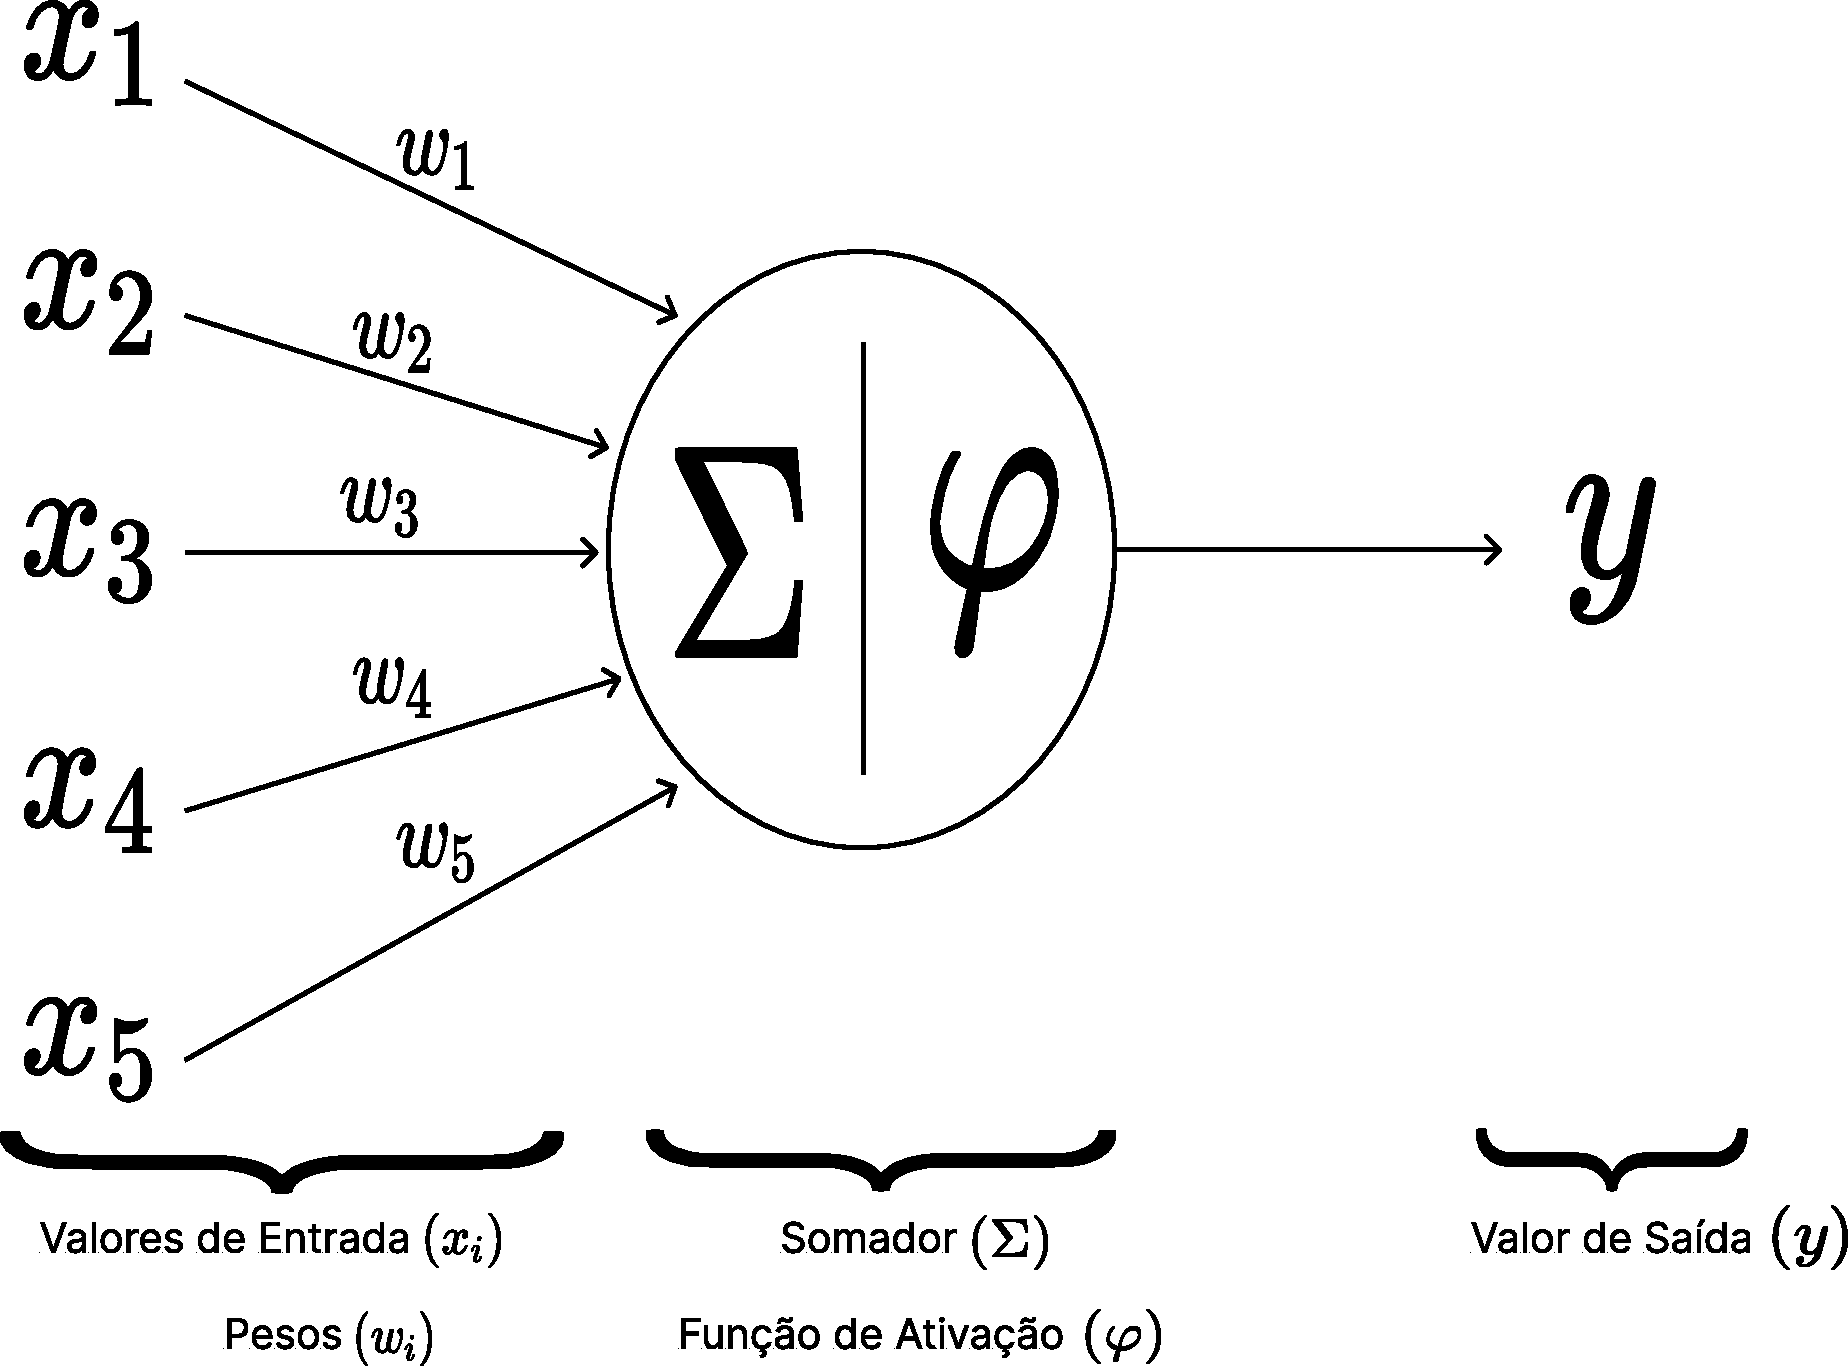
\includegraphics[width=.7\textwidth]{figuras/neuron_model.pdf}
	\caption{Modelo Neuronal \citep[adaptado de][]{hair2005,haykin2009}}
\end{figure}

Dada uma sequência $x_1,\cdots,x_m$ de dados de entrada (valores observados) e uma função de ativação $\varphi(\cdot)$, a descrição do $k$-ésimo neurônio em uma rede neural nada mais é do que a determinação da função que leva o vetor de entrada $(x_1,\cdots,x_m)$ na $k$-ésima saída $y_k$. Uma configuração simples de um neurônio é dada pelo sistema de equações:
\begin{align}\label{vk}
    u_k & := \sum_{i=1}^{m} w_{k,i}x_i; \nonumber\\   
    y_k & := \varphi(u_k + b_k),
\end{align}
sendo $b_k$ o \textit{bias} e $w_{k,i} \in \R$ os pesos associados ao neurônio.



        % Função de Ativação
\subsection{Função de Ativação}
Uma função de ativação pode ser linear ou não linear. Seu objetivo em geral é transformar o valor de $v_k := u_k + b_k$ para um valor que esteja de acordo com a distribuição de $y_k$, como pode ser visto em \eqref{vk}. A escolha de uma particular função de ativação depende do problema que o neurônio almeja resolver. Em problemas de classificação de classe binária, ela é responsável por levar o valor de $v_k \in \R$ para o intervalo $(0,1)$, possibilitando a predição das respectivas classes. Abaixo, seguem alguns exemplos:
\begin{itemize}
    \item \textbf{linear:} $f: \R \rightarrow \R$ dada por 
    \[f(x) := \alpha x, \quad \alpha \in \R\backslash\{0\}.\]
    Observe que no caso da função linear, o neurônio está sempre ativado, sendo seu valor alterado pela constante $\alpha$. Em particular, quando $\alpha=1$, temos a função identidade e, consequentemente, um modelo de regressão linear.
    \item \textbf{sigmóide ou \textit{logit}}: $f: \R \rightarrow (0,1)$ dada por 
    \[f(x) := \frac{1}{1 + e^{-x}}.\]
    Quando essa função de ativação é associada a uma rede, o neurônio é equivalente a uma regressão logística. Dessa forma, notamos que a função de ativação tem um papel semelhante à função de ligação no contexto de modelos lineares generalizados: relacionar o preditor linear ao respectivo valor esperado \citep{sarle1994,frei2020,mccullagh1989}.
    \item \textbf{tangente hiperbólica (\textit{tanh}):}  $f:\R \rightarrow (-1,1)$ dada por 
    \[f(x) := \frac{e^{x}-e^{-x}}{e^{x}+e^{-x}}.\]
    Em contextos que uma função sigmoidal é necessária (como a predição de uma variável binária), a \textit{tanh} tipicamente performa melhor. Vale comentar que funções de ativação sigmoidais são mais comuns em estruturas diferentes que a de redes alimentadas adiante, como as redes recorrentes \citep{goodfellow2016}.  
    \item \textbf{ReLU (\textit{Rectified Linear Unit}):} $f: \R \rightarrow [0,\infty)$ dada por 
    \[f(x) := \max\{0,x\}.\]
    De acordo com \citet{goodfellow2016}, é a recomendação padrão para redes neurais modernas. O autor justifica que, por ser uma função quase linear, são preservadas muitas propriedades que fazem os modelos lineares bons generalizadores. 
    \item \textbf{\textit{softmax}}: $f:\R^n\rightarrow (0,1)^n$ dada por 
    \[f(\bs x):=\bigg(\frac{e^{x_1}}{\sum_{j=1}^n e^{x_j}},\cdots, \frac{e^{x_n}}{\sum_{j=1}^n e^{x_j}}\bigg), \quad \forall\,\bs x=(x_1,\cdots,x_n)\in\R^n.\]
    {A função} é tipicamente utilizada para transformar vetores reais em vetores a ser interpretados como probabilidades, bastante útil em problemas de classificação.
\end{itemize}
Listas de funções de ativação comumente utilizadas podem ser encontradas em \citet{hastie2008}, \citet{hagan2014}, \citet{aggarwal2018} e \citet{dsa2022}.



        % Arquitetura de RNAs
\subsection{Arquiteturas de RNAs}
\label{arquitetura rna}

Um único neurônio, mesmo com muitas entradas, usualmente não é suficiente para resolver problemas complexos, sendo necessários por vezes diversos operando paralelamente em uma estrutura que chamamos de ``camada''. Temos que uma rede neural é constituída por três tipos básicos de camadas:

\begin{enumerate}
    \item \textbf{entrada:} constituída por nós de fonte, em que cada nó representa uma variável independente. Vale comentar que variáveis numéricas requerem apenas um nó, porém variáveis categóricas requerem um nó para cada categoria, semelhantemente ao processo de criação de variáveis dicotômicas ou \textit{dummies}, mas sem a eliminação de uma categoria de referência.
    \item \textbf{saída:} composta por neurônios, com a diferença que seu valor de saída é definitivo. No caso de um modelo preditivo, o valor será o resultado da previsão. Se o modelo é utilizado para classificação, então o valor resultante será empregado no processo de classificação (que será utilizado para determinar qual categoria foi classificada).
    \item \textbf{intermediária ou oculta:} assim como a camada de saída, é composta por neurônios. Seus valores de entrada podem ser originados da camada de entrada ou da camada oculta anterior, bem como seus valores de saída podem alimentar a próxima camada oculta ou a camada de saída.
\end{enumerate}
Posto isso, organizamos as redes em três arquiteturas fundamentalmente diferentes \citep{hair2005,haykin2009,hagan2014}: redes alimentadas adiante com camada única, com múltiplas camadas e redes recorrentes.



            % Redes Alimentadas Adiante
\subsubsection{Redes Alimentadas Adiante}
A nomenclatura desse tipo de arquitetura é devida ao fluxo de informação partir da camada de entrada até a camada de saída, de forma unidirecional \citep{goodfellow2016}. \citet{hastie2008} e \citet{fan2021} comentam que é o tipo padrão de rede neural. A principal diferença entre uma rede de camada única e uma com múltiplas camadas é a existência (ou não) das camadas ocultas, sendo que a designação ``camada única'' se refere a uma camada de neurônios. Além disso, há a distinção entre a rede ser totalmente ou parcialmente conectada, no sentido de que os nós de uma camada são conectados a todos os nós da camada adjacente ou não \citep{haykin2009}. 

\begin{figure}[ht!]
    \centering
    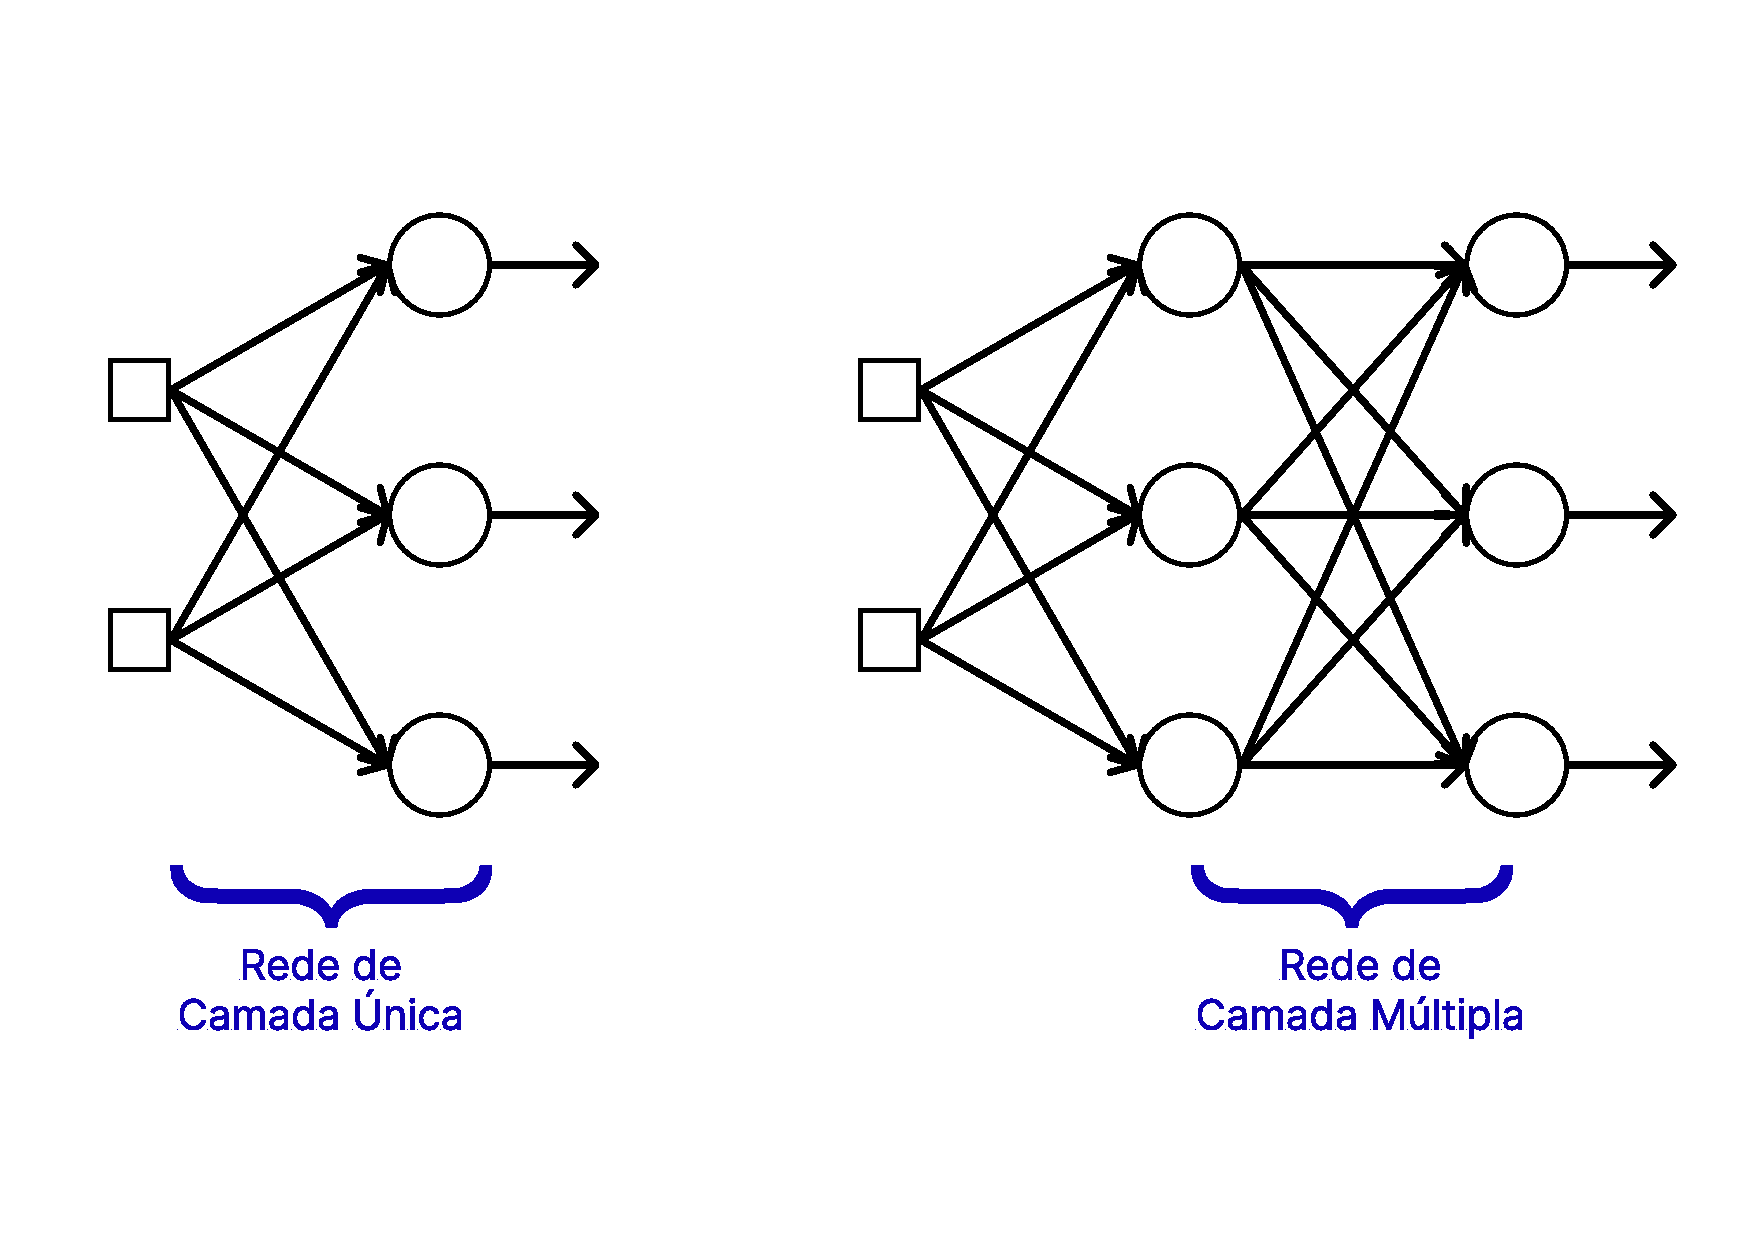
\includegraphics[width=.7\textwidth]{figuras/network_layers.pdf}
	\caption{Rede Camada Única e Múltipla \citep[adaptado de][]{haykin2009}}
\end{figure}

\begin{figure}[ht!]
    \centering
    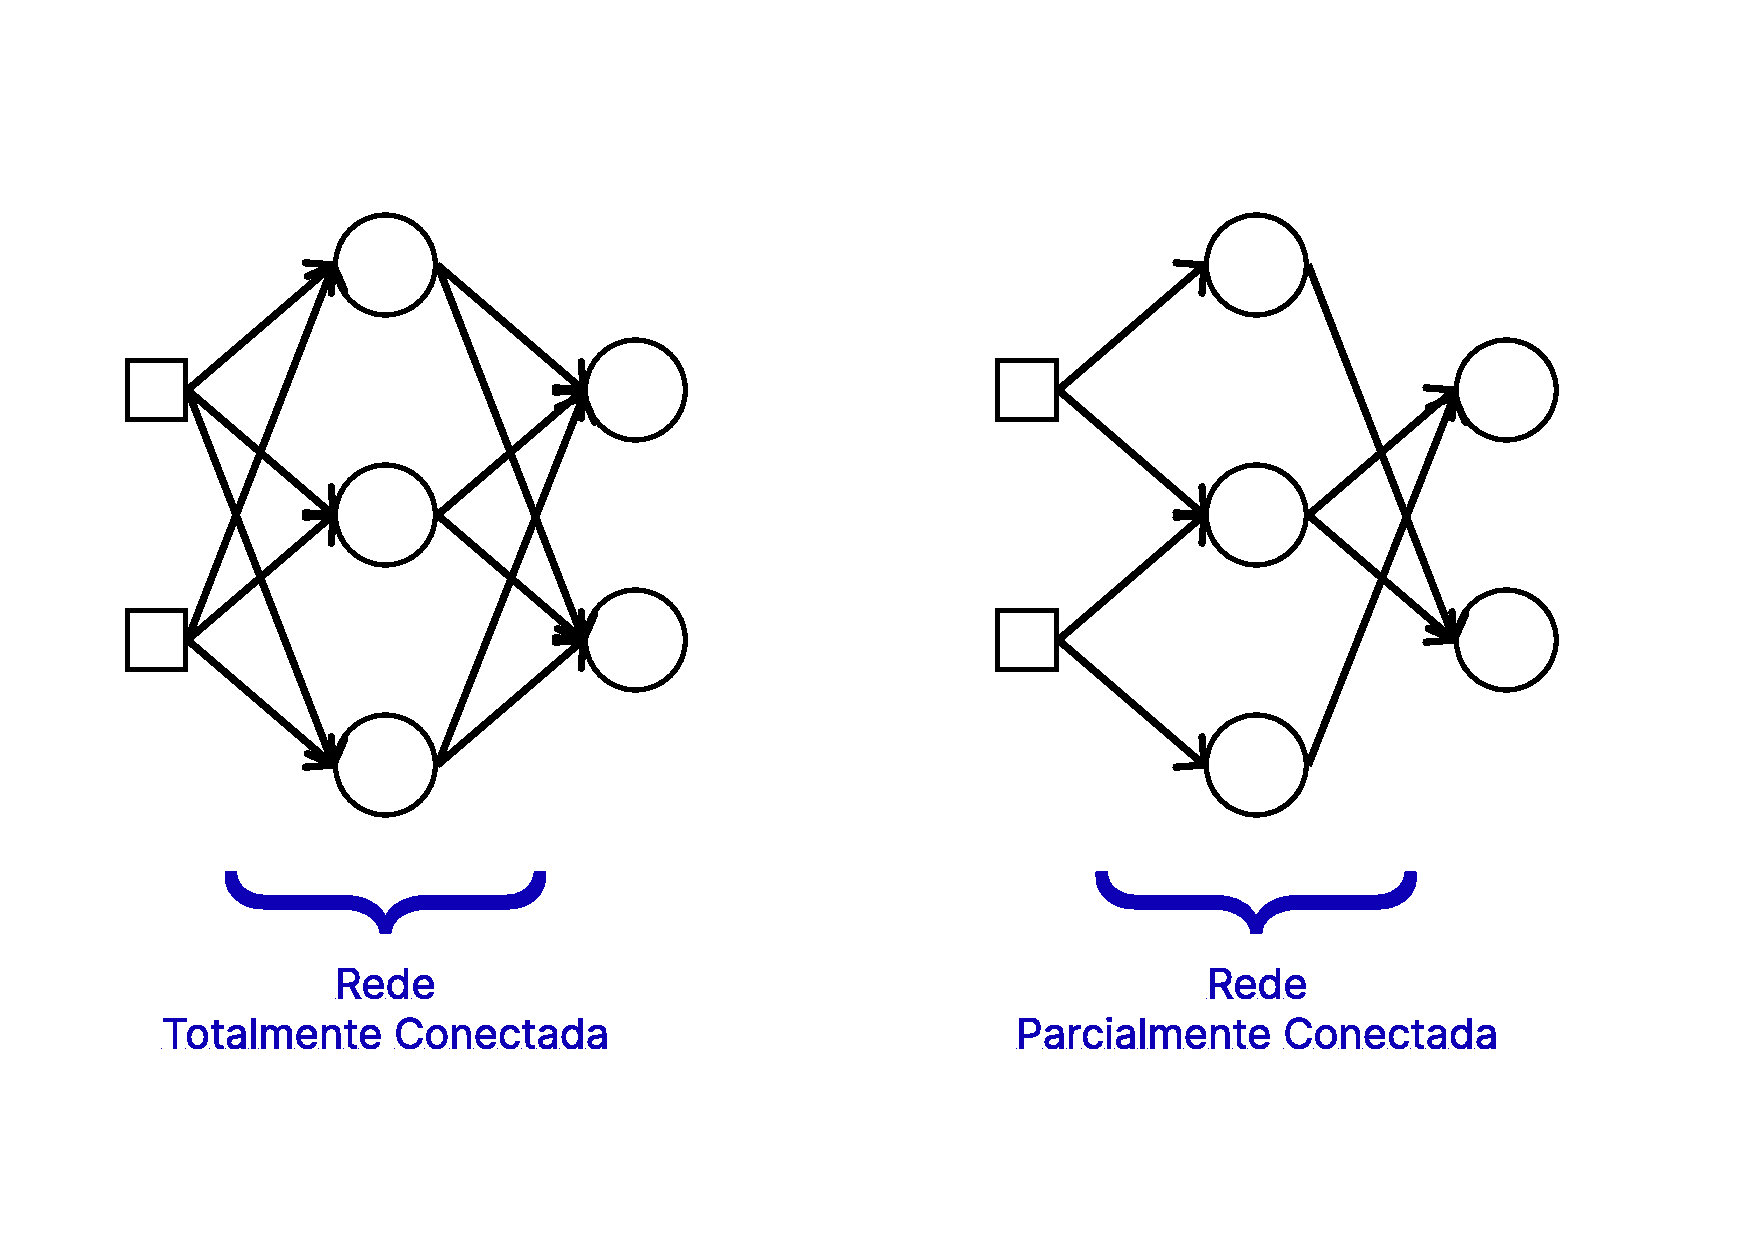
\includegraphics[width=.7\textwidth]{figuras/network_connections.pdf}
	\caption{Rede Totalmente e Parcialmente Conectada \citep[adaptado de][]{haykin2009}}
\end{figure}


            
            % Redes Neurais Recorrentes
\subsubsection{Redes Neurais Recorrentes}
Redes neurais recorrentes (RNNs) são um tipo de redes neurais criadas para processar séries temporais e outros tipos de dados sequenciais \citep{fan2021}. O que difere uma rede recorrente de uma rede alimentada adiante é seu laço de realimentação. Por exemplo, uma rede recorrente pode consistir de uma única camada de neurônios com cada neurônio alimentando seu sinal de volta para as entradas de todos os outros neurônios \citep{haykin2009}. 



            % RNN Vanilla    
\subsubsection{RNN \textit{Vanilla}}
Sejam $\bs{x}_{1},\cdots,\bs{x}_{n}$ dados de entrada. Uma  RNN \textit{vanilla} modela o estado oculto (\textit{hidden state}) $\bs{h}_{t}$ via
\begin{equation*}
    \bs{h}_t = f_{\bs{{\theta}}} (\bs{h}_{t-1}, \bs{x}_{t}),    
\end{equation*}
em que $f_{\bs{\theta}}$ geralmente é uma função não linear parametrizada por $\bs{\theta}$. Assim como em modelagem de séries temporais, há o compartilhamento dos parâmetros ao longo do tempo.

Dada uma sequência de entrada $\bs{x}_{t},\cdots,\bs{x}_{1}$, pode-se utilizar $\bs{h}_{t}$ para fazer predições. Por exemplo, se a RNN é utilizada para modelagem estatística de linguagem (como prever as próximas palavras dadas as palavras anteriores), não é necessário armazenar todas as informações na sequência de entrada até o tempo $t$, apenas o suficiente para prever o resto da sentença.

\begin{figure}
    \centering
    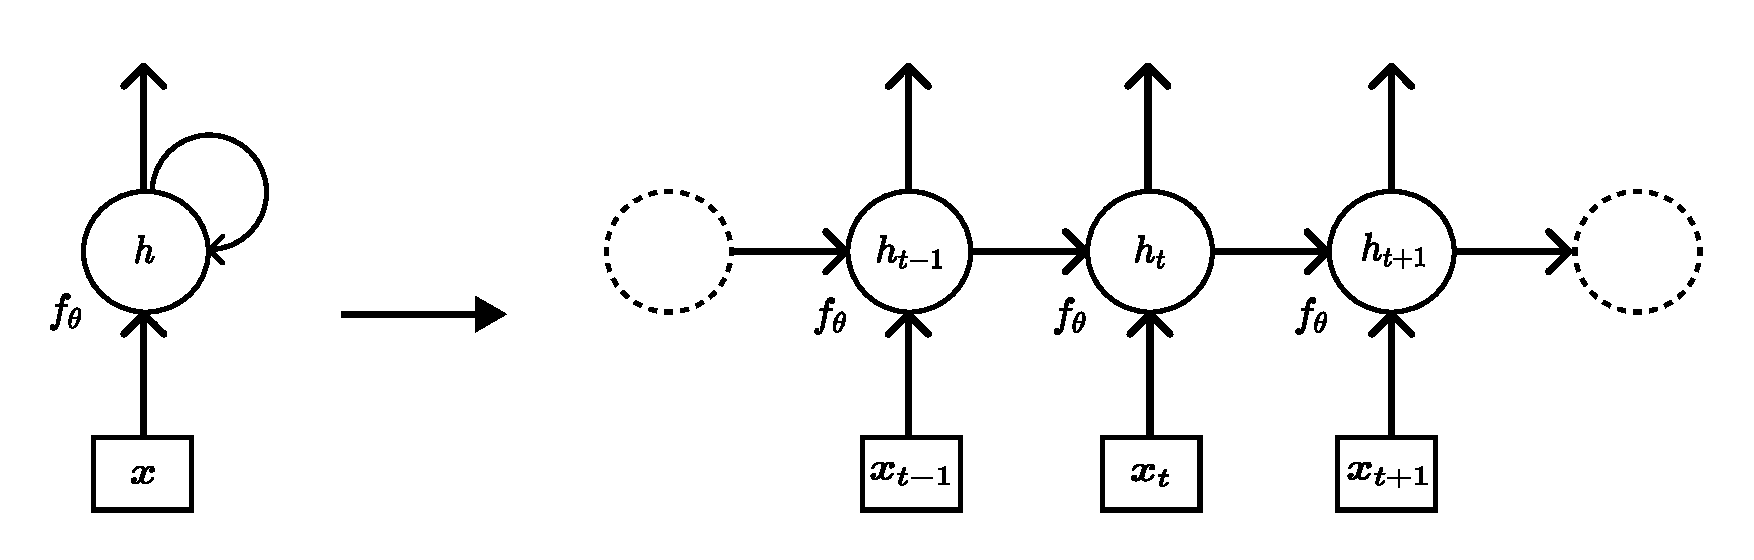
\includegraphics[width=\textwidth]{figuras/rnn_hidden_state.pdf}
	\caption{Diagrama de uma RNN \textit{Vanilla} \citep[adaptado de][]{goodfellow2016, kamath2019}}
\end{figure}

Um déficit da RNN \textit{vanilla} é sua dificuldade em capturar longa dependência nos dados. Esse problema é comumente relacionado ao fenômeno de dissipação (ou explosão) do gradiente, que ocorre no ajuste da rede. Dentre as variantes desenvolvidas para contornar esse problema, destacaremos a \textit{long short-term memory} \citep{goodfellow2016, fan2021}.



            % LSTM   
\subsubsection{LSTM - \textit{Long Short-Term Memory}}
De acordo com \citet{goodfellow2016}, as LSTM fazem parte de uma classe de modelos chamada de RNN fechadas (\textit{gated RNN}). Os portões (\textit{gates}), que também são camadas da rede neural, controlam o fluxo de informação, mantendo ou descartando o estado oculto $\bs{h}_{t}$ a cada passo temporal \citep{kamath2019}. 

Denote por $\odot$ o produto de Haddamard, isto é, a multiplicação por elemento (\textit{element-wise multiplication}). O estado de célula $\bs{c}_t$ carrega informações da sequência (por exemplo, forma singular ou plural de uma sentença). O portão de esquecimento (\textit{forget gate}) $\bs{f}_t$ determina por quanto tempo os valores de $\bs{c}_{t-1}$ são mantidos, o portão de entrada (\textit{input gate}) $\bs{i}_t$ controla a quantidade de atualizações realizadas no estado de célula, e o portão de saída (\textit{output gate}) $\bs{o}_t$ define quanta informação $\bs{c}_t$ revela para $\bs{h}_t$, de forma que a arquitetura da rede se torna 
\begin{align*}
    \bs{c}_{t} & = \bs{f}_{t} \odot \bs{c}_{t-1} + \bs{i}_{t} \odot \bs{h}_{t}, \\
    \bs{h}_{t} & = \bs{o}_{t} \odot \varphi(\bs{c}_{t}),
\end{align*}
em que $\varphi(\cdot)$ é uma função de ativação, usualmente a \textit{tanh}. Além disso, os elementos desses portões têm valores no intervalo $(0,1)$, sendo utilizada a função de ativação \textit{logit} para garantir isso. O estado de célula $\bs{c}_t$ tem uma adição em sua fórmula, o que auxilia o algoritmo de retropropagação e, portanto, captura-se longa dependência nos dados \citep{goodfellow2016, fan2021}.

\begin{figure}[H]
    \centering
    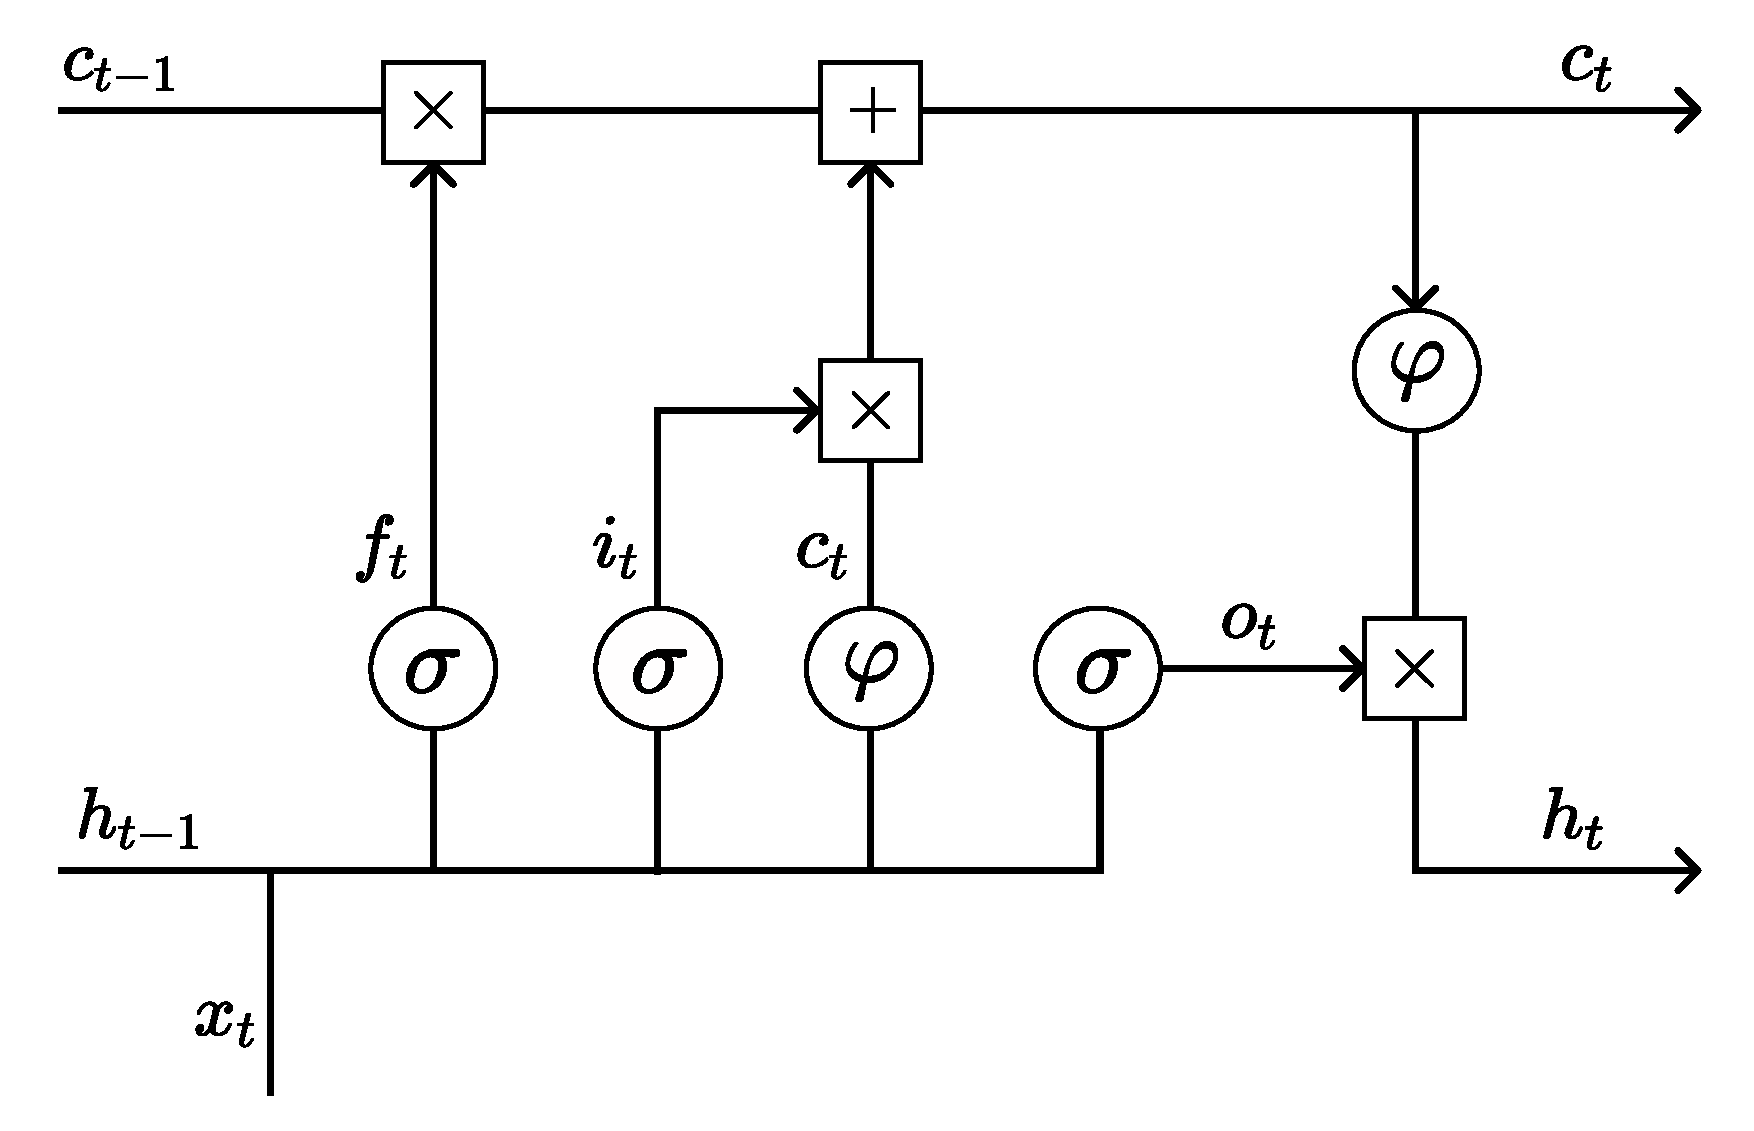
\includegraphics[width=\textwidth]{figuras/lstm_cell.pdf}
	\caption{Diagrama de uma LSTM. Considere $\sigma$ como a função de ativação \textit{logit} \citep[adaptado de][]{kamath2019}.}
\end{figure}

Entende-se, portanto, que o diferencial de uma LSTM em relação a RNN \textit{vanilla} são as suas ``células LSTM'' (\textit{LSTM cells}), que contêm uma recorrência interna (\textit{self-loop}), além da recorrência existente da RNN. Sendo assim, cada célula possui as mesmas entradas e saídas de uma RNN, mas há mais parâmetros e um sistema de portões controlando o fluxo de informação \citep{goodfellow2016}.


        % Ajustando uma RNA
\subsection{Ajustando uma RNA}
Algoritmos de aprendizagem de máquina, usualmente, envolvem alguma parte de otimização, referindo-se a minimizar (ou maximizar) uma função $f(x)$. Tal função pode ser chamada de \textbf{função custo} (\textit{cost function}) ou de \textbf{função perda} (\textit{loss function}). 


Seja $f: \R^n \rightarrow \R^n$ uma função diferenciável, e denote por $\nabla_{\bs{x}} f(\bs{x})$ o gradiente de $f$ no ponto $\bs{x}\in\R^n$. Os pontos críticos de $f$ são as soluções das equações $\nabla_{\bs{x}} f(\bs{x}) = \bs{0}$, em que $\bs{0}$ denota o valor nulo em $\R^n$. Posto isso, podemos minimizar $f$ por meio do método  do gradiente descendente (\textit{\textbf{gradient descent}}), também conhecido como \textit{\textbf{steepest descent}}, propondo um novo ponto
\begin{equation*}
    \bs{x'} = \bs{x} - \epsilon \nabla_{\bs{x}} f(\bs{x}),
\end{equation*}
em que $\epsilon$ é chamada de \textbf{taxa de aprendizagem} (\textit{learning rate}), um escalar positivo que determina o tamanho do passo em termos do valor do gradiente no ponto. O método converge quando todos os elementos do gradiente ficam abaixo de uma tolerância predeterminada \citep{goodfellow2016}. 

Uma das desvantagens  do método do gradiente descendente é o uso de todo o conjunto de treino para o cálculo do gradiente. Devido a isso, a  gradiente descendente estocástico (\textbf{\textit{stochastic gradient descent} - SGD}) utiliza uma partição aleatória dos dados, denominada lote (\textbf{\textit{minibatch}}). Iniciando com um certo valor $\bs{\theta}_0$, o SGD ajusta os parâmetros $\bs{\theta}_t$ em direção ao gradiente negativo, e utilizando uma partição aleatória dos dados de forma iterativa para minimizar uma função perda. Pela Lei dos Grandes Números, o SGD aproxima-se do gradiente calculado. Por fim, temos que uma passagem pelo conjunto de dados de treinamento é denominada \textbf{época} (\textit{epoch}), e após um determinado número de épocas, o treinamento é concluído \citep{goodfellow2016, kamath2019, fan2021}. 

ADAM (\textit{adaptive moment estimation}) é um método de otimização do SGD direcionado a problemas de aprendizagem de máquina com grandes conjuntos de dados ou com espaço paramétrico com muitas dimensões. O método combina as vantagens do AdaGrad \citep{duchi2011} de lidar com esparsidade de gradientes (gradientes iguais a zero) e as vantagens do RMSProp \citep{tieleman2012} de lidar com não estacionariedade. O detalhamento destes métodos fogem ao escopo deste trabalho. Mais informações podem ser encontradas em \citet{kingma2014}.

O algoritmo de retropropagação (\textbf{\textit{back-propagation}}) permite que a informação da função de custo flua para trás através da rede neural, com o intuito de calcular o gradiente. O termo ``retropropagação'' refere-se ao método de calcular o gradiente e, por meio do SGD, os parâmetros da rede neural (no caso, os pesos) são ajustados. No contexto de RNN, os gradientes são calculados considerando, também, o índice $t \in T$ e, nesse caso, o algoritmo é chamado de retropropagação ao longo do tempo (\textbf{\textit{back-propagation through time} - BPTT}). Maiores detalhes podem ser encontrados em \citet{haykin2009}, \citet{goodfellow2016} e \citet{fan2021}.  



    % Processamento de Linguagem Natural
\section{Processamento de Linguagem Natural}
O objetivo da ciência linguística é ser capaz de caracterizar e de explicar as diversas observações linguísticas ao nosso redor, presentes em conversações, na escrita e em outras mídias. Parte disso está relacionado à compreensão das estruturas linguísticas pelas quais a linguagem se comunica e, devido a isso, foram propostas regras para a estruturação das expressões linguísticas. Tal abordagem tornou-se cada vez mais formal e rigorosa à medida que os linguistas exploravam gramáticas detalhadas que tentavam descrever o que seria um texto bom ou mau escrito \citep{manning1999}.

Processamento de Linguagem Natural (PLN), também conhecida como Linguística Computacional, foca na aplicação de métodos quantitativos e estatísticos para entender como seres humanos modelam linguagem, bem como abordagens computacionais para responder perguntas linguísticas. Ou seja, é a aplicação de métodos computacionais para modelar e extrair informações da linguagem humana \citep{kamath2019}. 

De acordo com \citet{jurafsky2021}, é importante testar algoritmos em mais de uma linguagem, especialmente em linguagens com diferentes propriedades. Em contraste, segundo \citet{bender2019}, há uma infeliz tendência atual: algoritmos de PLN serem desenvolvidos apenas em inglês. Mesmo quando algoritmos são desenvolvidos para outras linguagens, eles tendem a serem desenvolvidos para idiomas oficiais de grandes nações industrializadas (chinês, espanhol, alemão, etc.), limitando essas ferramentas. Vale também destacar que o texto em que essas ferramentas serão aplicadas podem ser oriundos de fontes como notícias, livros, artigos científicos, reuniões de negócios, transcrições de programas televisivos ou filmes, textos jurídicos, entre outros. Em sumo, ainda segundo \citet{jurafsky2021}, é importante considerar quem produziu a linguagem, em qual contexto e para qual propósito.



        % Corpus e Corpora
\subsection{Corpus e Corpora}
Um \textit{corpus} (plural \textit{corpora}) é uma coleção de material textual (seja em um único documento ou uma coleção de documentos) construído de acordo com algum critério. Esse material é constituído com ao menos uma linguagem escrita (representação via símbolos de uma linguagem falada ou gestual). Em PLN, comumente temos um \textit{corpus} com uma determinada quantidade de dados de algum domínio de interesse (como discursos, material literário, conversas em redes sociais, entre outros), sem necessariamente ter algum tipo de opinião de como ele foi construído. Dentre os cuidados que devemos ter ao selecionar um \textit{corpus} ou ao relatar os resultados obtidos nas análises são se o tipo de texto é representativo ou se os resultados obtidos são úteis para o domínio de interesse \citep{manning1999, kamath2019}.



        % Expressões Regulares
\subsection{Expressões Regulares}
Expressões Regulares são particularmente úteis para pesquisar em textos, localizando determinados padrões em um \textit{corpus}. \citet{jurafsky2021} comentam que, formalmente, uma expressão regular é uma notação algébrica utilizada para caracterizar um conjunto de \textit{strings}. Além disso, uma função de busca com expressões regulares pode ser projetada para retornar todas as correspondências ao padrão definido, bem como apenas a primeira. Por fim, detalhamentos e demais definições referentes a expressões regulares estão disponíveis em \citet{jurafsky2021}.



        % Vocabulário e Tokenização
\subsection{Vocabulário e Tokenização}
Tokenização é o processo computacional de segmentar texto em unidades denominadas \textit{tokens}, podendo ser palavras, números ou sinais de pontuação. Em seu processo mais simples, tokenização pode ser realizada ao separar texto por espaços em branco, induzindo um vocabulário ou um dicionário \citep{kamath2019, jurafsky2021}.

Segundo \citet{manning1999}, um método comumente utilizado em PLN é o mapeamento de palavras e de seus tokens para números (realizando a conversão do número para caractere quando necessário). Dentre as formas de realizar esse mapeamento, podemos citar uma tabela \textit{hash} (uma função \textit{hash} mapeia um conjunto de objetos para um intervalo específico de inteiros não negativos), que conterá um conjunto de \textit{tokens} e seus respectivos índices. Por meio de tal tabela, pode-se obter tanto os índices quanto os \textit{tokens} quando necessário.



        % Modelos de Linguagem
\subsection{Modelos de Linguagem}
Um modelo estatístico de linguagem é aquele que atribui probabilidades para uma sequência de \textit{tokens}. Por exemplo, pode-se determinar a probabilidade de uma determinada sequência por meio da probabilidade de cada \textit{token} disponível nos \textit{tokens} anteriores. Dentre suas aplicações, tem-se reconhecimento de fala, tradução automática, marcação de parte da fala (\textit{part-of-speech tagging}), reconhecimento de manuscrito, recuperação de informação, entre outras
\citep{kamath2019, jurafsky2021}.




        % Avaliação Intrínseca e Extrínseca
\subsection{Avaliação Intrínseca e Extrínseca}
Existem dois tipos de avaliação de um modelo de linguagem: extrínseca e intrínseca. Uma avaliação \textbf{extrínseca} envolve encapsular o modelo em uma aplicação e medir se houve melhorias. Por exemplo, em um contexto de reconhecimento de fala, o texto transcrito seria comparado com o discurso realizado. Apesar da avaliação extrínseca verificar qual ajuste melhora o desempenho do modelo, desenvolver um sistema completo para tal objetivo é usualmente caro, afetando sua viabilidade. Uma alternativa é a avaliação \textbf{intrínseca}, que consiste em utilizar uma métrica objetiva para mensurar as potenciais melhorias do modelo de linguagem. Basicamente, é um tipo de avaliação que mede a qualidade de um modelo independentemente de sua aplicação. No entanto, uma melhora na métrica intrínseca não necessariamente implica em uma melhora na avaliação extrínseca. 

No caso de uma avaliação intrínseca de um modelo de linguagem, assim como em muitos modelos estatísticos, realizamos o ajuste por meio de um conjunto de treino, e medimos a qualidade do modelo pelo seu desempenho no conjunto de teste. Dado um \textit{corpus}, podemos dividi-lo em treino e teste por meio de sequências de \textit{tokens} (como palavras ou caracteres) presentes em partes sorteadas do texto. Mais detalhes podem ser encontrados em \citet{goldberg2017} e \citet{jurafsky2021}.




        % Entropia e Perplexidade
\subsection{Entropia e Perplexidade}
\label{entropia e perplexidade}

Seja $p(w)$ a função massa de probabilidade de uma variável aleatória discreta $W$, associada a um conjunto de \textit{tokens} (ou vocabulário) $L$. A \textbf{entropia} mede a quantidade de informação de uma variável aleatória, sendo definida por
\begin{equation*}
    H(p) := -E \big(\log \big( p(W)\big) \big) = - \sum_{w \in L} p(w) \log \big(p(w)\big). 
\end{equation*}
No contexto de uma sequência de palavras de tamanho $n$, digamos $W_1, \cdots, W_n$, calcula-se a taxa de entropia (\textit{entropy rate})  por
\begin{equation*}
    H_{rate} := - \frac{1}{n} \sum_{\bs{w} \in L^n} p(\bs{w}) \log \big(p(\bs{w})\big). 
\end{equation*}

Quando a verdadeira massa de probabilidade $p$ que gerou os dados é desconhecida, pode-se utilizar a \textbf{entropia cruzada} (\textit{cross-entropy}) para aproximar a entropia. Seja $m$ um estimador para $p$ (por exemplo, a massa de probabilidade empírica), a entropia cruzada é definida pela expressão
\begin{equation*}
    H(p,m) := \lim_{n \rightarrow \infty}  - \frac{1}{n} \sum_{\bs\omega \in L^n}  p(\bs{w}) \log\big(m(\bs{w})\big) .
\end{equation*}
Quando o processo estocástico $H(p,m)$ é estacionário e ergótico, podemos aproximá-lo via
\begin{equation*}
    H(p,m) = \lim_{n \rightarrow \infty} \; - \frac{1}{n} \sum_{\bs\omega \in L^n} \log\big(m(\bs{w})\big).
\end{equation*}
A intuição é que uma sequência de palavras suficientemente longa conterá outras sequências menores, e que cada uma dessas irá ocorrer recorrentemente na sequência mais longa de acordo com suas respectivas probabilidades.

É interessante observar que a entropia cruzada $H(p,m)$ é o limite superior da entropia $H(p)$. Devido a isso, temos que
\begin{equation*}
    H(p) \leq H(p,m).
\end{equation*}
Isso indica que pode-se utilizar $m$ para estimar a verdadeira entropia de uma sequência de \textit{tokens} gerados por $p$. Quanto maior for a acurácia de $m$, mais próximo $H(p,m)$ será de $H(p)$. Dessa forma, ao comparar dois estimadores, $m_1$ e $m_2$, o melhor será aquele com a menor entropia cruzada.

\textbf{Perplexidade} é uma medida oriunda da teoria da informação, comumente utilizada para a avaliação intrínseca de um modelo de linguagem, definida como
\begin{align*}
    \Perp (W) := e^{H(\bs{W})} = p(\bs{w})^{-\frac{1}{n}}.
\end{align*}
Medidas menores de perplexidade são indicativas de uma predição melhor. Por fim, é importante destacar que a perplexidade de dois modelos de linguagem apenas podem ser comparadas se ambos utilizam o mesmo vocabulário (\textit{corpus}). Maiores informações são encontradas em \citet{manning1999}, \citet{kamath2019} e \citet{jurafsky2021}.



        % Word Embedding
\subsection{Word Embedding}
Em PLN, as palavras (ou \textit{tokens}) são variáveis categóricas que precisam de uma codificação para que sejam utilizadas em um modelo estatístico. Seguem duas possibilidades:
\begin{itemize}
    \item \textit{one-hot encoding}: é criado uma variável indicadora (\textit{dummy}) para cada categoria.
    \item \textit{dense encoding (feature embeddings)}: cada categoria é embutida em um vetor $d$-dimensional.
\end{itemize}
O principal benefício da \textit{dense encoding} é a capacidade de generalização, pois os valores do vetor denso são ajustáveis, possibilitando a captura de relações entre as diferentes palavras.

No contexto de RNA, podemos utilizar vetores esparsos (\textit{one-hot encoding}) na camada de entrada e uma camada embutida (\textit{embedding layer}) para obter o vetor denso que representará as categorias. Matematicamente, cada categoria $f_i$ é mapeada a um vetor denso $d-$dimensional $\bs v(f_i)$. Seja um vocabulário de $|V|$ palavras, a coleção de vetores pode ser representada pela matriz $\bs{E}_{|V| \times d}$, em que cada linha corresponde a uma categoria. Considere $\bs{f_i}$ a representação \textit{one-hot} da categoria $f_i$, i.e., um vetor $|V|$ dimensional em que todas os valores são zeros exceto por um índice de valor 1, correspondente à $i$-ésima categoria. Dessa forma, o produto $\bs{f_i E}$ irá ``selecionar'' a respectiva linha de $\bs{E}$. Posto isso, podemos definir $\bs v(f_i)$ como
\begin{equation*}
    \bs v(f_i) = \bs{f_i E}.
\end{equation*}
em que a entrada da rede é a coleção de vetores \textit{one-hot}. Apesar de elegante e bem definido matematicamente, uma implementação computacional eficiente não utiliza essa representação, mas sim uma estrutura de dados estilo tabela \textit{hash}, mapeando cada categoria a seu respectivo vetor denso \citep{goldberg2017}.



        % Notação ABC
\section{Notação ABC}
Notação ABC é um sistema popular de notação musical baseada em texto para transcrever, publicar e compartilhar músicas folclóricas, particularmente de forma \textit{online}. Criada e formalizada por \citet{walshaw1993}, o autor mantém um website, \href{https://abcnotation.com}{\url{abcnotation.com}}, com recursos como tutoriais, programas e coleções de músicas no formato \citep{walshaw2014}.

A notação ABC é composta por duas partes: o cabeçalho, que fornece os metadados da música como o título e características da música, e o corpo, que detalha as notas musicais. Existem \textit{tags} no cabeçalho como ``T'' (título) e ``X'' (número da música) que não afetam a síntese musical de nenhuma forma. Vale notar que a notação ABC define um mapeamento entre seus caracteres e símbolos específicos de uma partitura musical, o que permite a conversão de um formato para outro \citep{agarwala2017}. 

\begin{figure}[H]
    \centering
    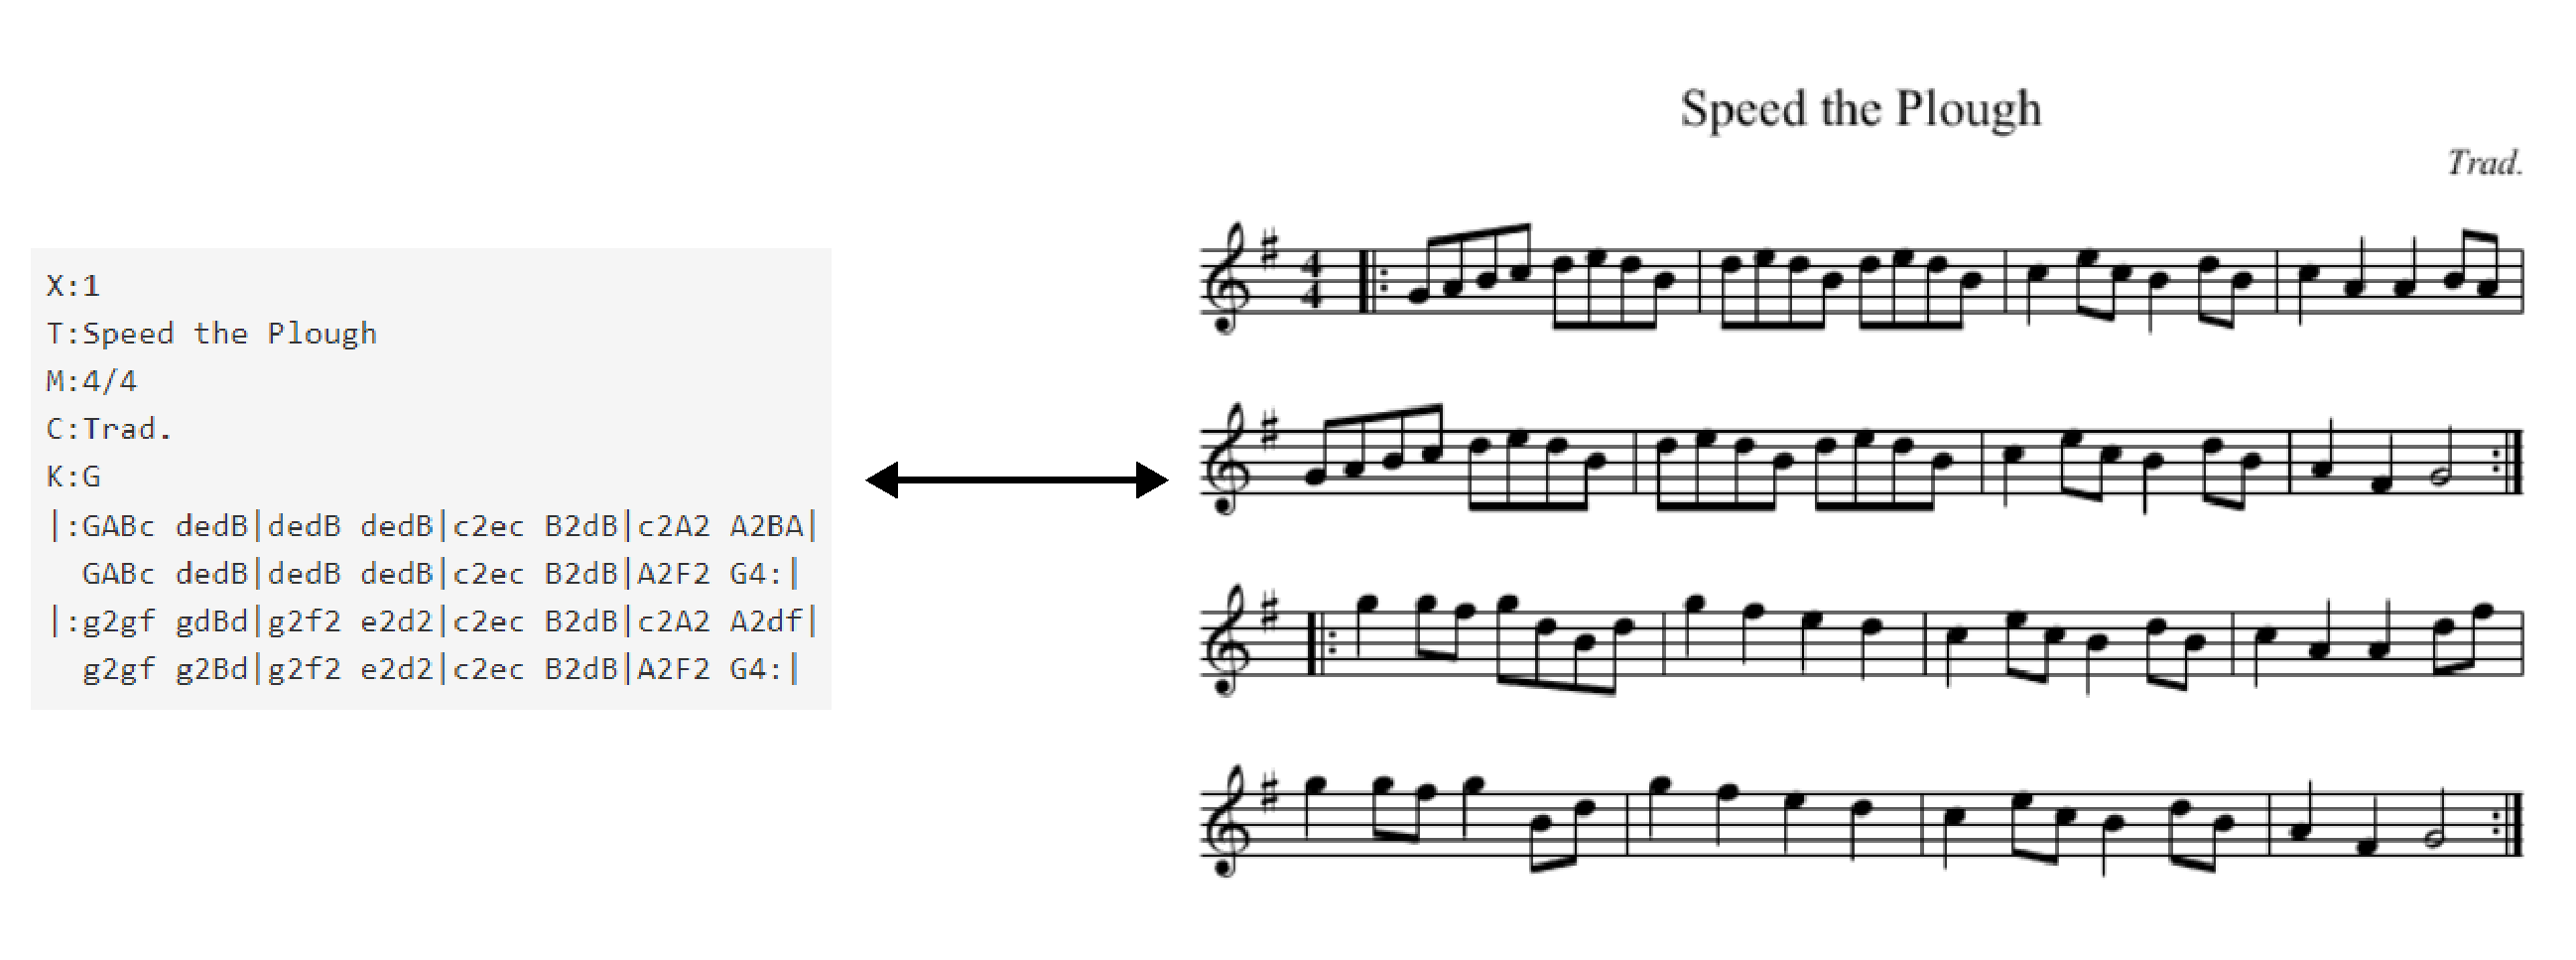
\includegraphics[width=\textwidth]{figuras/abc_notation_example.pdf}
	\caption{Exemplo de notação ABC convertendo em música (disponível em \href{https://abcnotation.com}{\url{abcnotation.com}}).}
\end{figure}


        % Web Scraping
\section{Web Scraping}
\textit{Web scraping} é uma técnica de extração automática de dados de fontes online como \textit{websites} \citep{farley2017,khder2021}. Seu desenvolvimento envolve dois programas customizados: um \textit{crawler} e um \textit{scraper}. O \textit{crawler} sistematicamente coleta os dados da Internet (especificamente, cria uma réplica da página visitada). Já o \textit{scraper} extrai a informação relevante dos dados baixados e os armazena em uma base de dados, no formato e estrutura definidos pelo usuário \citep{lawson2015,patil2016}.

Grande parte dos \textit{websites} contém um arquivo \textit{robots.txt} para informar sobre quaisquer restrições sobre o uso da técnica em seus domínios. Essas restrições são apenas sugestões, mas é recomendado que sejam seguidas, pois além de poderem conter informações sobre a estrutura do \textit{website}, minimiza a chance do \textit{crawler} ser bloqueado. Mais informações sobre o arquivo \textit{robots.txt} estão disponíveis em \url{robotstxt.org} \citep{lawson2015}.

Dentre as linguagens comumente utilizadas para o desenvolvimento do \textit{crawler} e do \textit{scraper} podemos citar \href{https://cran.r-project.org}{R} e \href{https://python.org/}{Python}. Detalhamentos sobre o assunto podem ser encontrados em \citet{lawson2015}, \citet{sirisuriya2015}, \citet{patil2016}, \citet{farley2017} e \citet{khder2021}.



%%%%%%%%%%%%%%%%%%%%%%%%%%%%%%%%%%%
%%%%  Modelagem
%%%%%%%%%%%%%%%%%%%%%%%%%%%%%%%%%%%
\chapter{Estudo de Modelagem}
O estudo de modelagem visa a explorar o impacto de diferentes configurações de uma rede neural utilizada para composição musical. Ao modificar os parâmetros e hiperparâmetros, serão observados os impactos no ajuste da rede, bem como na métrica selecionada. Por fim, os diferentes modelos gerarão novas peças musicais, que serão avaliadas de forma subjetiva dado o desafio de mensurar uma música.



        % Implementação Computacional
\section{Implementação Computacional}
\label{computacional}

O processo de obtenção de dados, bem como os modelos utilizados nesse trabalho foram desenvolvidos na linguagem de programação \href{https://python.org/}{Python} e na IDE (\textit{Integrated Development Environment}) \href{https://code.visualstudio.com}{VS Code}. As bibliotecas utilizados neste trabalho foram as seguintes:
\begin{itemize}
    \item \textbf{Python}: versão 3.9.12;
    \item \href{https://www.tensorflow.org/?hl=pt-br}{\textbf{TensorFlow}}: versão 2.9.1;
    \item \href{https://numpy.org}{\textbf{NumPy}}: versão 1.22.3;
    \item \href{https://pypi.org/project/regex/}{\textbf{regex}}: versão 2.5.112;
    \item \href{https://scikit-learn.org/stable/}{\textbf{sklearn}}: versão 1.1.1;
    \item \href{https://pypi.org/project/beautifulsoup4/}{\textbf{bs4}}: versão 4.10.0;
    \item \href{https://pypi.org/project/requests/}{\textbf{requests}}: versão 2.27.1;
    \item \href{https://web.mit.edu/music21/}{\textbf{music21}}: versão 7.3.3.
\end{itemize}
Além disso, as análises dos resultados foram realizados na linguagem \href{https://cran.r-project.org}{R} e na IDE \href{https://www.rstudio.com}{RStudio}:
\begin{itemize}
    \item \textbf{R}: versão 4.1.2;
    \item \href{https://ggplot2.tidyverse.org}{\textbf{ggplot2}}: versão 3.3.5;
    \item \href{https://patchwork.data-imaginist.com}{\textbf{patchwork}}: versão 1.1.2;
    \item \href{https://dplyr.tidyverse.org}{\textbf{dplyr}}: versão 1.0.8.
\end{itemize}
Por fim, todos os códigos desenvolvidos nesse trabalho estão disponíveis em um repositório no \href{https://github.com/nmhahn/TCC_NMH}{GitHub do autor}.



        % Bases de Dados
\section{Bases de Dados}
O trabalho foi realizado utilizando duas bases de dados: Irish e ABC Notation. Abaixo, seguem algumas explicações sobre cada uma:
\begin{itemize}
    \item \textbf{Irish}: base de dados contendo 817 músicas folclóricas irlandesas no formato \textit{.abc}. Foi utilizada a versão disponibilizada pelo Instituto de Tecnologia de Massachusetts (MIT) em seu \href{https://github.com/aamini/introtodeeplearning/blob/master/mitdeeplearning/data/irish.abc}{GitHub}. No entanto, existem mais exemplos de fontes de músicas no formato como pode ser visto \href{https://www.norbeck.nu/abc/links.asp}{nesta página}.
    \item \textbf{ABC Notation}: inspirado pelo artigo de \citet{agarwala2017}, o autor quis realizar sua própria coleta de músicas no formato \textit{.abc} do site \href{https://abcnotation.com/}{abcnotation.com}. Foi desenvolvido, na linguagem Python, um \textit{crawler} e um \textit{scrapper} para a obtenção dos dados. Após uma semana de execução, foram obtidos 184.900 arquivos no formato desejado contendo diversas informações referentes às peças musicais (como título, autor, tonalidade da música, entre outras). Por conseguinte, foi selecionada uma amostra aleatória simples de 5.000 músicas dessa base.
\end{itemize}
Depois, ambas as bases de dados utilizadas passaram por três procedimentos: tratamento, união e tokenização. Abaixo, alguns detalhes sobre cada uma:
\begin{itemize}
    \item \textbf{tratamento}: um arquivo no formato \textit{.abc} contém diversas \textit{tags} com informações como título, subtítulo, autor, entre outras. Além disso, no arquivo também estão contidos caracteres representando letra de música, bem como caracteres de comentário. Como nenhuma desses itens afetam diretamente a música, considerando que as notas musicais serão as mesmas, o autor resolveu, por meio de expressões regulares, remover esses caracteres, com o intuito de diminuir o ruído nos arquivos. Após os tratamentos, o arquivo final contém dados como índice (representando o início da música), tonalidade, andamento, vozes da música (no caso de músicas com múltiplos instrumentos) e as notas musicais (mantendo a estrutura da peça musical).
    \item \textbf{união}: todas as músicas foram ``coladas'', como se fizessem parte de um único texto. Esse processo possibilita que uma música inicie após o término da outra, pois temos, de certa forma, uma ordem de músicas (no caso, foi a ordem presente na base, sem aleatorização).
    \item \textbf{tokenização}: para cada caractere (\textit{token}) presente, foi criado um único índice. Consequentemente, é possível que uma sequência de caracteres seja convertido para uma sequência única de índices, possibilitando a conversão de texto para número e vice-versa.
\end{itemize}




    % Modelo
\section{Modelo}
Utilizou-se um modelo de RNN-LSTM, que foi ajustado com ambas as bases de dados de forma independente, ou seja, tem-se uma versão com a base Irish e outra com a base ABC Notation. Esse modelo não é original do autor, pois foi desenvolvido no \href{https://goodboychan.github.io/python/tensorflow/mit/2021/02/14/music-generation.html\#The-Recurrent-Neural-Network-(RNN)-model}{laboratório de geração musical} ministrado pelo MIT. Além disso, foi feita uma divisão dos dados em 80\% treino e 20\% teste. No entanto, todo o processo de tratamento foi realizado antes dessa divisão.



        % Arquitetura
\subsection{Arquitetura}
Como elucidado na seção \ref{arquitetura rna}, uma rede neural é constituída de camadas de neurônios e de nós de fonte. O modelo utilizado contém quatro camadas: entrada, \textit{Embedding}, LSTM e \textit{Dense}. A primeira contém o vocabulário (conjunto de \textit{tokens}), sendo único para cada base. A segunda é responsável pelo \textit{dense encoding}, identificando as possíveis relações entre os \textit{tokens}. A terceira contém os neurônios LSTM, responsáveis pelo mapeamento temporal da sequência de elementos. Por fim, na última camada encontram-se as saídas da rede, sendo os resultados preditos.



        % Parâmetros e Ajuste da Rede
\subsection{Parâmetros e Ajuste da Rede}
O processo de modelagem foi feito utilizando 2000 épocas no ajuste do modelo, tendo a entropia cruzada como função perda e a perplexidade como métrica de avaliação. Ademais, houve uma segmentação em duas etapas. Na primeira etapa, foi fixada a função de ativação \textit{tanh} na camada LSTM, alterando-se os demais parâmetros e hiperparâmetros: 
\begin{itemize}
    \item o tamanho do vocabulário: \textit{vocab\_size}, sendo $64$ para \textit{Irish} e $125$ para \textit{ABC Notation};
    \item número de células LSTM: \textit{lstm\_units} $\in \{256,1024\}$;
    \item a dimensão do vetor utilizado para \textit{dense encoding}: \textit{embedding\_dim} $\in \{256,512\}$;
    \item a taxa de aprendizagem no ajuste: \textit{learning\_rate} $\in \{10^{-3},10^{-5}\}$;
    \item comprimento da sequência obtida dos dados: \textit{seq\_length} $\in \{50,200\}$;
    \item tamanho do lote sorteado do texto único, via amostra aleatória simples sem reposição: \textit{batch\_size} $\in \{4,16\}$.
\end{itemize}
Consequentemente, foram ajustados 64 modelos, sendo 32 para cada base de dados. A segunda etapa do experimento consistiu em trocar a função de ativação para a \textit{logit}, e avaliar se houveram mudanças na perplexidade dos modelos. Devido ao volume de modelos, alterou-se apenas os dois piores e os dois melhores em termos da perplexidade.




        % Processo Gerador de Músicas
\subsection{Processo Gerador de Músicas}
Tendo os modelos devidamente ajustados, foi possível realizar a composição algorítmica de novas peças musicais. O processo gerador consiste de cinco passos:
\begin{enumerate}
    \item construir um modelo com os devidos parâmetros (\textit{vocab\_size}, \textit{lstm\_units}, \textit{embedding\_dim} e \textit{batch\_size}), mas fixar $batch\_size=1$ para que haja apenas um vetor de entrada e um de saída; 
    \item fixado o modelo, carregam-se os pesos de um modelo similar ajustado previamente, sendo a única diferença entre eles o parâmetro \textit{batch\_size};
    \item o processo gerador envolve fornecer uma sequência de caracteres inicial, neste trabalho foi fornecida ``X:'', pois é como qualquer música presente no arquivo \textit{.abc} inicia;
    \item de forma iterativa, o modelo estima um novo elemento para compor a sequência até atingir um comprimento definido (no caso, utilizou-se 1000);
    \item via expressões regulares, são extraídos da sequência blocos de texto candidatos a músicas e, ao serem convertidos com sucesso, resultam em músicas.
\end{enumerate}




%%%%%%%%%%%%%%%%%%%%%%%%%%%%%%%%%%%
%%%%  Resultados
%%%%%%%%%%%%%%%%%%%%%%%%%%%%%%%%%%%
\chapter{Resultados}
Cada base de dados será avaliada individualmente, considerando as diferentes configurações de parâmetros definidas e os impactos em ambas função perda (entropia cruzada) e métrica de avaliação (perplexidade). Como comentado na seção \ref{entropia e perplexidade}, dois modelos de linguagem são comparáveis apenas se compartilharem o mesmo vocabulário (único por base). Após, será explanado sobre as (potenciais) músicas geradas, bem como as percepções subjetivas do autor. 



    % Irish
\section{Irish}
Inicialmente, avaliou-se a primeira etapa do estudo. A tabela \ref{table:irish_tanh_full} contém os resultados dos 32 modelos ajustados (identificados pela coluna \textit{idx}) para a base de dados Irish, bem como os respectivos parâmetros e função de ativação \textit{tanh}. Além disso, a figura \ref{fig:irish_tanh_loss} inclui a função perda calculada para cada época do ajuste. 

De maneira geral, observou-se certos padrões no comportamento da função perda de acordo com a configuração da rede:
\begin{itemize}
    \item No geral, o aumento do \textit{batch\_size} resultou na redução dos valores da função perda, bem como em uma menor variabilidade a cada época. Tal comportamento é coerente, dado que há mais dados utilizados no treino.
    \item \textit{seq\_length} tem comportamento e justificativa similares ao \textit{batch\_size}.
    \item O impacto do \textit{learning\_rate} na função perda é evidente, acusando um aumento na perda quando a taxa de aprendizagem é menor. Isso ocorre, pois, ao ser calculado o gradiente, o passo foi demasiado pequeno para o processo de otimização. 
    \item O parâmetro \textit{embedding\_dim} não parece, em geral, afetar significativamente nos valores da função perda nos experimentos conduzidos.
    \item Aumentar os valores de \textit{lstm\_units}, geralmente, ocasionou em uma redução na função perda. 
\end{itemize}

A figura \ref{fig:irish_tanh_corr} apresenta a matriz de correlação entre os parâmetros e as métricas, sendo o $\rho$ de Spearman a medida de correlação. É notável que a matriz corrobora os padrões identificados. Destaque para a forte correlação negativa de $-0.87$ de \textit{learning\_rate} tanto com a perda quanto com a perplexidade. Ademais, é interessante notar que \textit{batch\_size} apresentou uma (fraca) correlação positiva com a perplexidade, sendo um indicativo de tendência a sobreajuste do modelo. 

\begin{figure}[!ht]
    \centering
    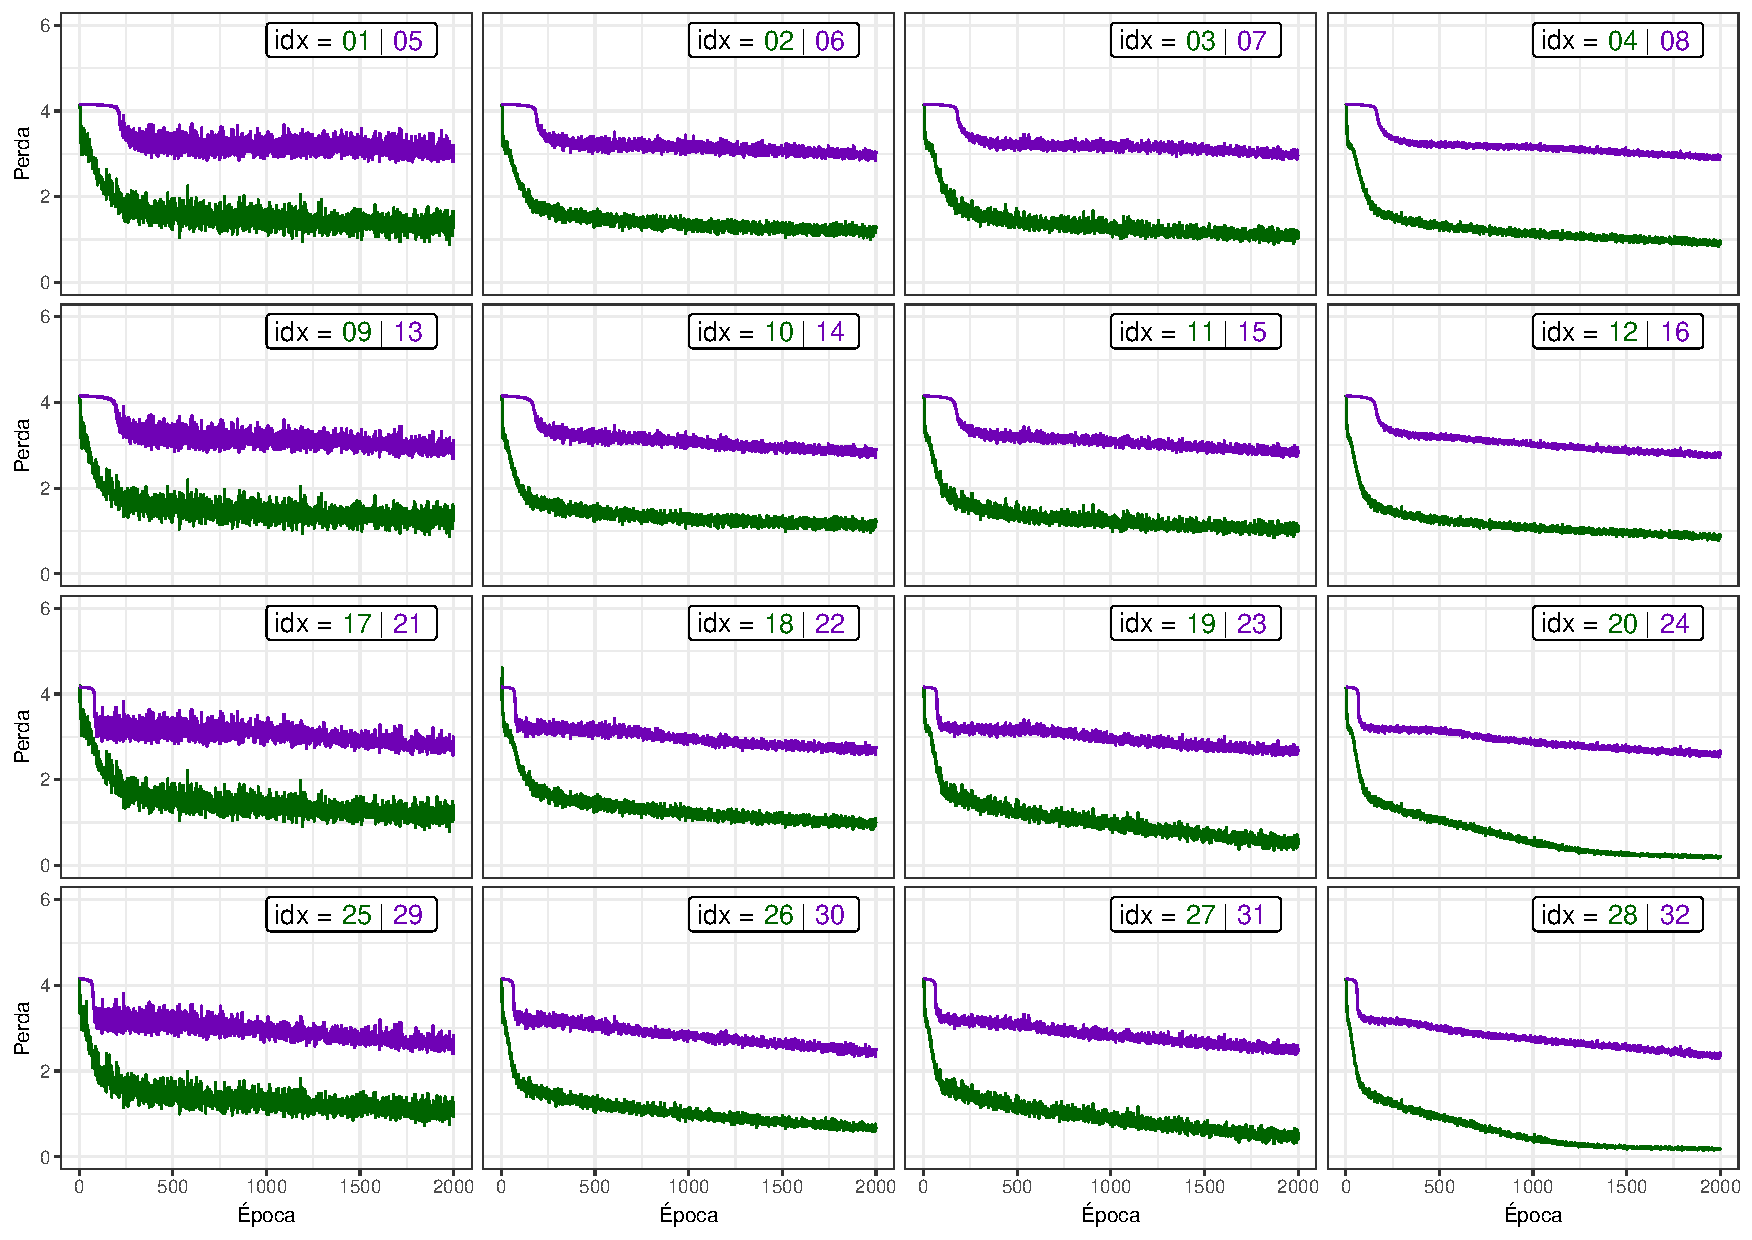
\includegraphics[width=\textwidth]{irish_tanh_loss.pdf}
    \caption{Perda dos modelos ajustados com Irish: curva verde representa $learning\_rate = 10^{-3}$ e roxo $learning\_rate = 10^{-5}$.}
    \label{fig:irish_tanh_loss}
\end{figure}

Na segunda etapa, os modelos selecionados, em ordem decrescente para perplexidade, foram $idx \in \{5,7,11,25\}$. Pela tabela \ref{tab:irish_tanh_vs_logit}, nota-se que as redes com função de ativação \textit{logit} tiveram um desempenho pior quando comparadas à \textit{tanh}.

\begin{figure}[H]
    \centering
    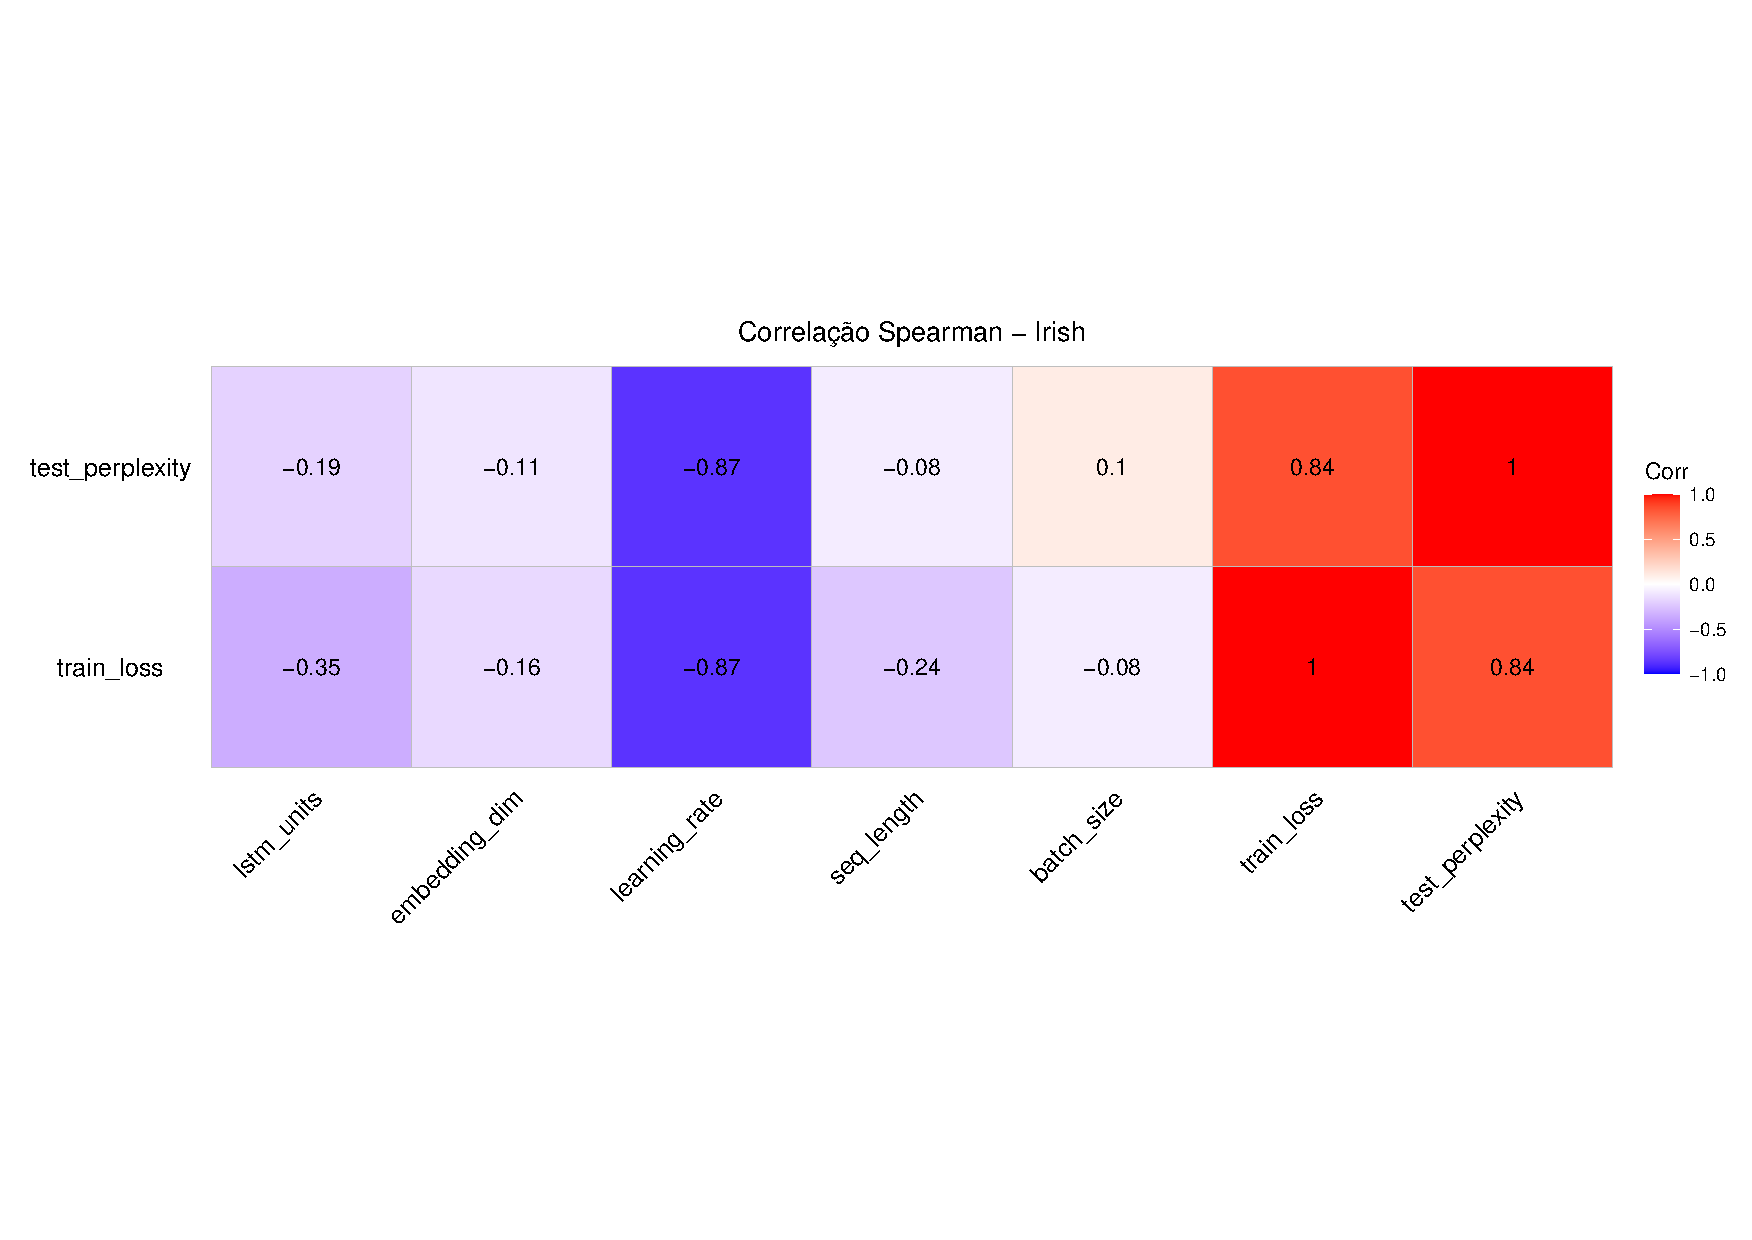
\includegraphics[width=\textwidth]{irish_tanh_corr.pdf}
    \caption{Correlação entre parâmetros e métricas para Irish}
    \label{fig:irish_tanh_corr}
\end{figure}

\rowcolors{2}{gray!25}{white}
\begin{table}[H]
    \caption{Resultados dos experimentos referentes à base de dados Irish, com $vocab\_size=64$, utilizando a função \textit{tanh} como função de ativação. Em azul (vermelho), constam os dois melhores (piores) modelos em relação à perplexidade.} 
    \label{table:irish_tanh_full}
    \centering
    \resizebox{\linewidth}{!}{
        \begin{tabular}[t]{ccccccccc}
        \toprule
        idx & lstm\_units & embedding\_dim & learning\_rate & seq\_length & batch\_size & train\_loss & test\_perplexity \\
        \midrule
        1 & 256 & 256 & $10^{-3}$ & 50 & 4 & 1.403 & 3.124 \\
        2 & 256 & 256 & $10^{-3}$ & 50 & 16 & 1.296 & 4.205 \\
        3 & 256 & 256 & $10^{-3}$ & 200 & 4 & 1.017 & 2.946 \\
        4 & 256 & 256 & $10^{-3}$ & 200 & 16 & 0.973 & 3.054 \\
        
        \red{5} & \red{256} & \red{256} & \red{$10^{-5}$} & \red{50} & \red{4} & \red{2.964} & \red{24.709} \\
        
        6 & 256 & 256 & $10^{-5}$ & 50 & 16 & 3.060 & 17.931 \\
        
        \red{7} & \red{256} & \red{256} & \red{$10^{-5}$} & \red{200} & \red{4} & \red{2.963} & \red{20.401} \\
        
        8 & 256 & 256 & $10^{-5}$ & 200 & 16 & 2.939 & 18.316 \\
        9 & 256 & 512 & $10^{-3}$ & 50 & 4 & 1.370 & 3.143 \\
        10 & 256 & 512 & $10^{-3}$ & 50 & 16 & 1.235 & 4.034 \\
        
        \blue{11} & \blue{256} & \blue{512} & \blue{$10^{-3}$} & \blue{200} & \blue{4} & \blue{0.982} & \blue{2.835} \\
        
        12 & 256 & 512 & $10^{-3}$ & 200 & 16 & 0.897 & 3.050 \\
        13 & 256 & 512 & $10^{-5}$ & 50 & 4 & 2.846 & 20.247 \\
        14 & 256 & 512 & $10^{-5}$ & 50 & 16 & 2.922 & 15.660 \\
        15 & 256 & 512 & $10^{-5}$ & 200 & 4 & 2.815 & 17.581 \\
        16 & 256 & 512 & $10^{-5}$ & 200 & 16 & 2.801 & 15.721 \\
        17 & 1024 & 256 & $10^{-3}$ & 50 & 4 & 1.298 & 2.896 \\
        18 & 1024 & 256 & $10^{-3}$ & 50 & 16 & 1.011 & 3.999 \\
        19 & 1024 & 256 & $10^{-3}$ & 200 & 4 & 0.615 & 2.884 \\
        20 & 1024 & 256 & $10^{-3}$ & 200 & 16 & 0.223 & 4.689 \\
        21 & 1024 & 256 & $10^{-5}$ & 50 & 4 & 2.692 & 16.002 \\
        22 & 1024 & 256 & $10^{-5}$ & 50 & 16 & 2.778 & 13.960 \\
        23 & 1024 & 256 & $10^{-5}$ & 200 & 4 & 2.645 & 14.593 \\
        24 & 1024 & 256 & $10^{-5}$ & 200 & 16 & 2.649 & 13.348 \\
        
        \blue{25} & \blue{1024} & \blue{512} & \blue{$10^{-3}$} & \blue{50} & \blue{4} & \blue{1.171} & \blue{2.752} \\
        
        26 & 1024 & 512 & $10^{-3}$ & 50 & 16 & 0.662 & 4.381 \\
        27 & 1024 & 512 & $10^{-3}$ & 200 & 4 & 0.567 & 3.019 \\
        28 & 1024 & 512 & $10^{-3}$ & 200 & 16 & 0.196 & 4.381 \\
        29 & 1024 & 512 & $10^{-5}$ & 50 & 4 & 2.522 & 13.508 \\
        30 & 1024 & 512 & $10^{-5}$ & 50 & 16 & 2.526 & 11.069 \\
        31 & 1024 & 512 & $10^{-5}$ & 200 & 4 & 2.460 & 12.176 \\
        32 & 1024 & 512 & $10^{-5}$ & 200 & 16 & 2.404 & 10.387 \\
        \bottomrule
        \end{tabular}
    }
\end{table}

Também, na figura \ref{fig:irish_tanh_vs_logit} são comparadas as curvas de perda dos modelos com cada função de ativação. Observou-se que o ajuste dos modelos com \textit{logit} apresentou um comportamento mais suave nos modelos $idx \in \{5,7\}$, não ocorrendo a mesma queda abrupta próxima da época 250 observada na \textit{tanh}. Por fim, pode-se concluir que a função \textit{tanh} apresentou melhores resultados para a base Irish.  

\rowcolors{3}{white}{gray!25}
\begin{table}[H]
    \caption{Irish: \textit{tanh} vs \textit{logit}} \label{tab:irish_tanh_vs_logit}
    \centering
    \begin{tabular}{c|cc|cc}
        \toprule
        \multirow{2}{*}{idx} &
        \multicolumn{2}{c|}{\textit{train\_loss}} &
        \multicolumn{2}{c}{\textit{test\_perplexity}} \\
        & {\textit{tanh}} & {\textit{logit}} & {\textit{tanh}} & {\textit{logit}} \\
        \midrule
        5 & 2.964 & 3.021 & 24.709 & 27.576 \\
        7 & 2.963 & 3.135 & 20.401 & 24.726 \\
        11 & 0.982 & 1.195 & 2.835 & 3.549 \\
        25 & 1.171 & 1.389 & 2.752 & 3.263 \\
    \bottomrule
  \end{tabular}
\end{table}

\begin{figure}[H]
    \centering
    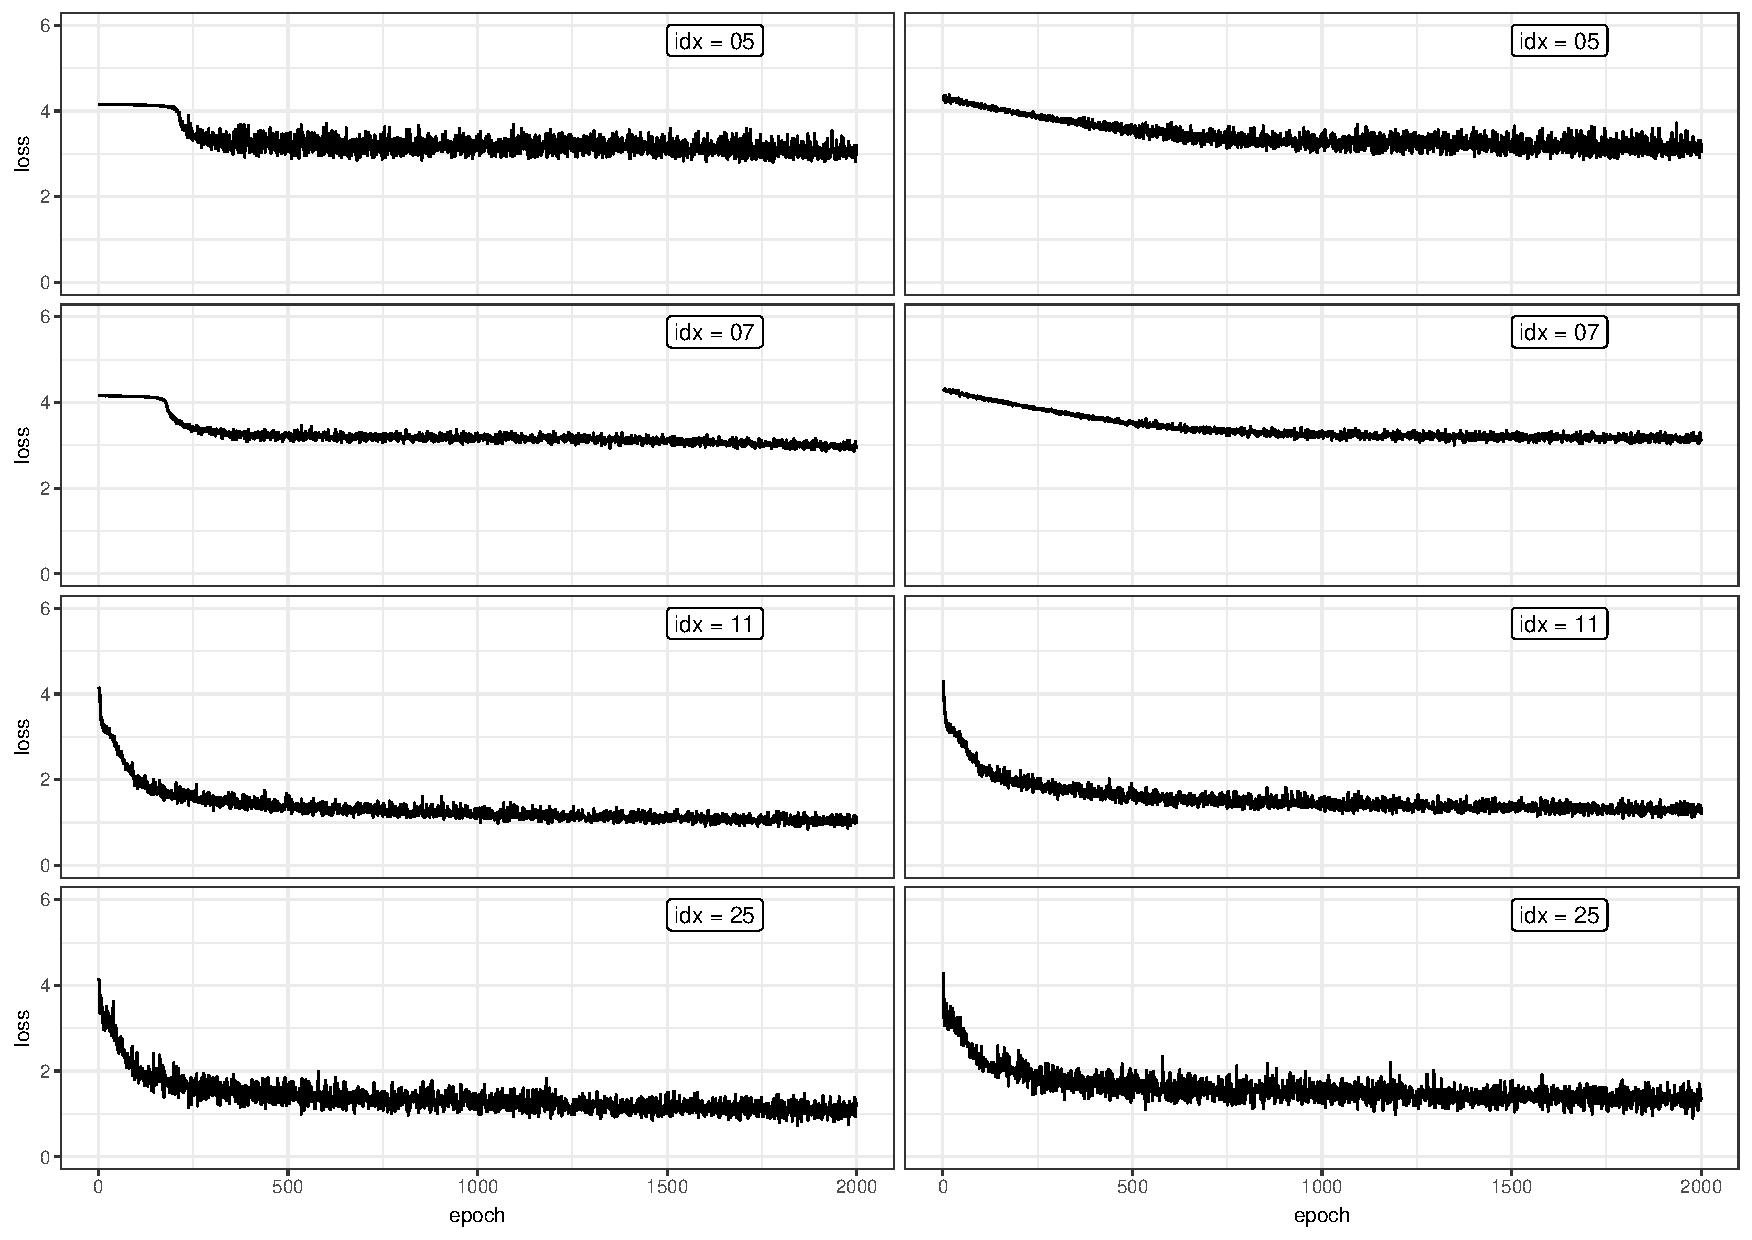
\includegraphics[width=\textwidth]{irish_tanh_vs_logit.pdf}
    \caption{Irish: \textit{tanh} (verde) vs \textit{logit} (roxo)}
    \label{fig:irish_tanh_vs_logit}
\end{figure}



    % ABC Notation
\section{ABC Notation}
Por meio de uma abordagem similar a Irish, avaliou-se a primeira etapa para os casos de ABC Notation. A tabela \ref{table:abcnotation_tanh_full} contém os resultados dos 32 modelos ajustados e na figura \ref{fig:abcnotation_tanh_loss} constam as perdas calculadas ao longo das épocas dos respectivos ajustes.




De maneira geral, observou-se certos padrões no comportamento da função perda com a modificação de acordo com a configuração da rede:
\begin{itemize}
    \item No geral, não é claro o impacto de \textit{batch\_size} na perda, mas permanece a redução de variabilidade a cada época.
    \item Diferentemente do observado em Irish, o aumento de \textit{seq\_length} apresentou, comumente, uma redução na função perda. Novamente, permanece a redução de variabilidade.
    \item Assim como notado em Irish, \textit{learning\_rate} tem um impacto expressivo na função perda, manifestando um aumento na perda quando a taxa de aprendizagem é menor. 
    \item O parâmetro \textit{embedding\_dim} continuou sem expor modificações significativas na função perda.
    \item Permanece o comportamento demonstrado em Irish para \textit{lstm\_units}. 
\end{itemize}
A figura \ref{fig:abcnotation_tanh_corr} apresenta a matriz de correlação entre os parâmetros e as métricas, sendo o $\rho$ de Spearman a medida de correlação. Uma vez mais, a matriz corrobora os padrões identificados, assim como a forte correlação negativa de $-0.87$ de \textit{learning\_rate} com a perda e com a perplexidade. Ademais, é interessante notar que \textit{batch\_size} apresentou uma (fraca) correlação negativa com a perplexidade, sendo o oposto observado na base Irish.

\begin{figure}[!ht]
    \centering
    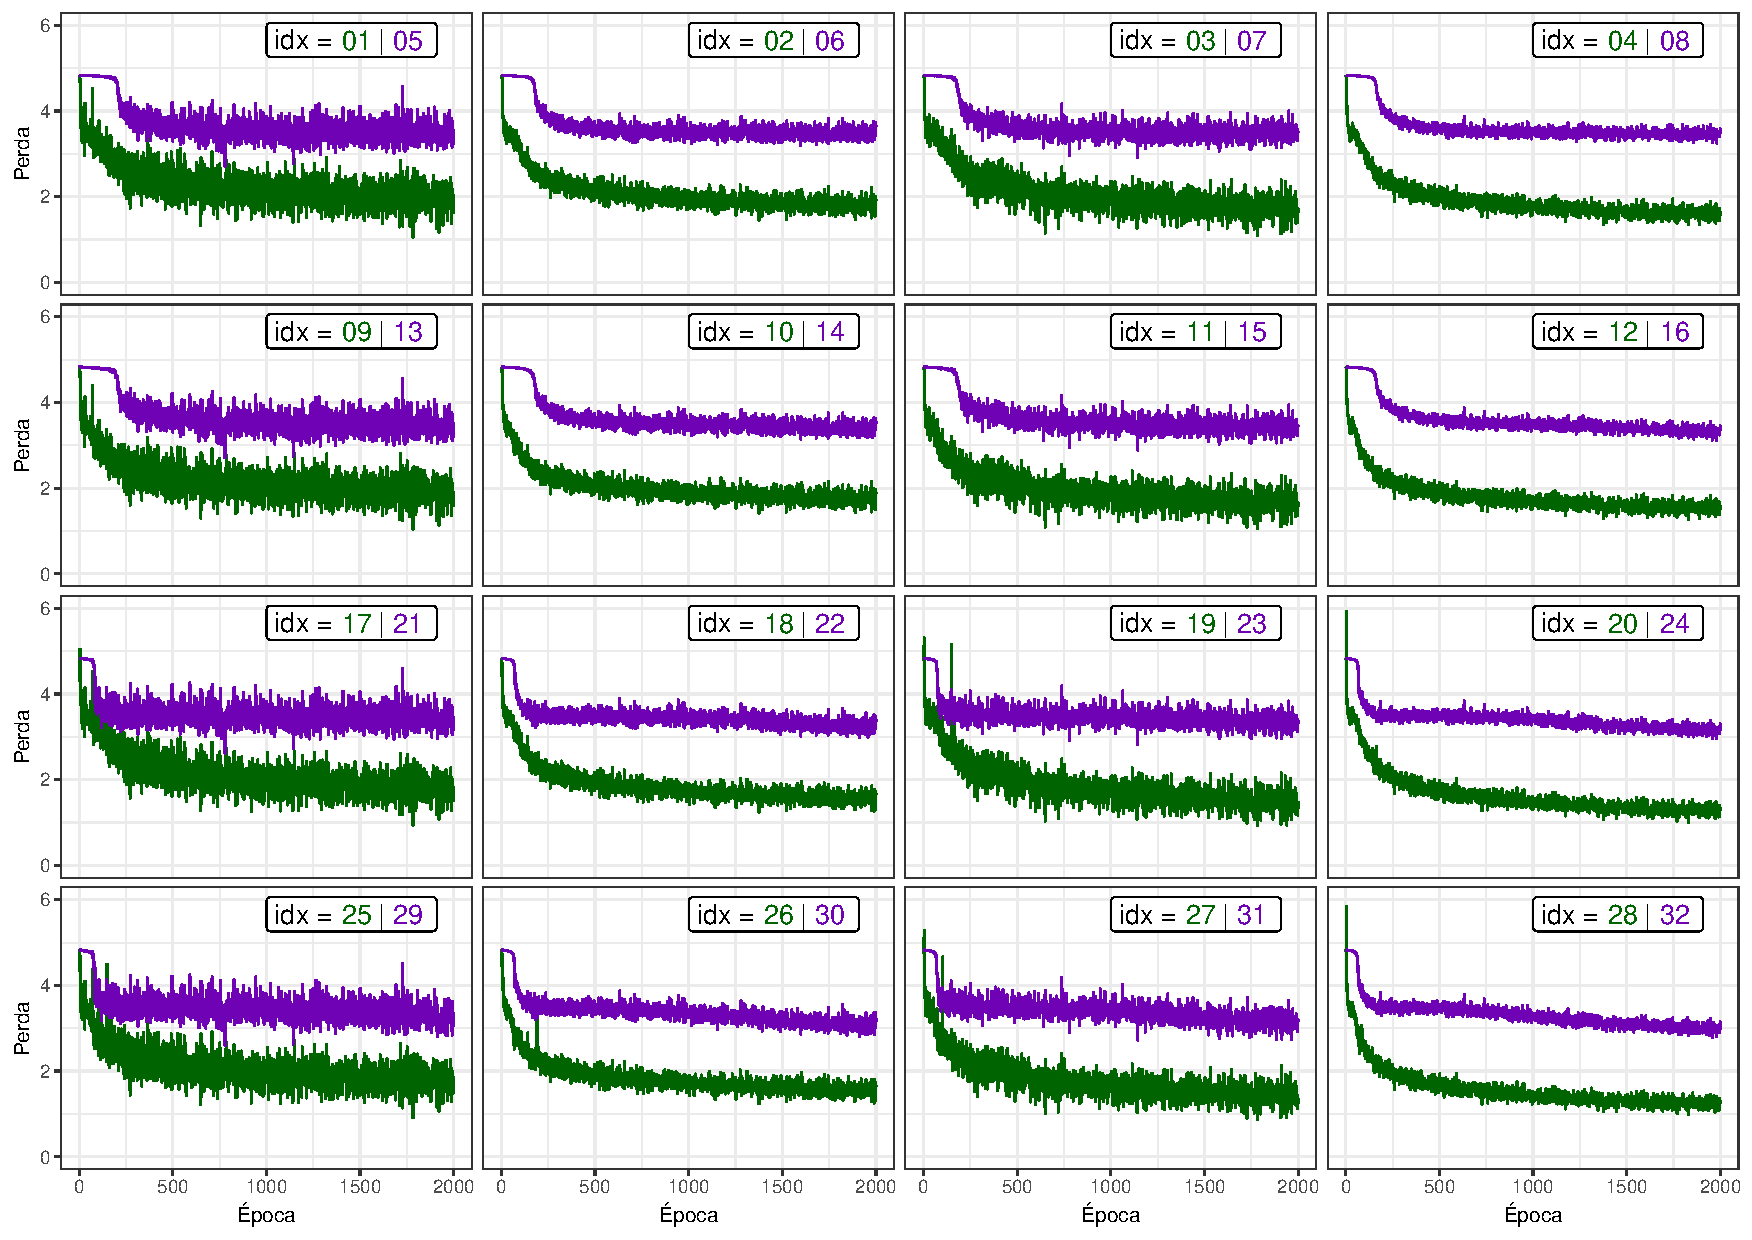
\includegraphics[width=\textwidth]{abcnotation_tanh_loss.pdf}
    \caption{Perda dos modelos ajustados com ABC Notation: curva verde representa $learning\_rate = 10^{-3}$ e roxo $learning\_rate = 10^{-5}$.}
    \label{fig:abcnotation_tanh_loss}
\end{figure}

Na segunda etapa, os modelos selecionados, em ordem decrescente para perplexidade, foram $idx \in \{8,6,20,28\}$. Pela tabela \ref{tab:abcnotation_tanh_vs_logit}, nota-se que as redes com função de ativação \textit{logit} tiveram um desempenho pior quando comparadas à \textit{tanh}.

\begin{figure}[H]
    \centering
    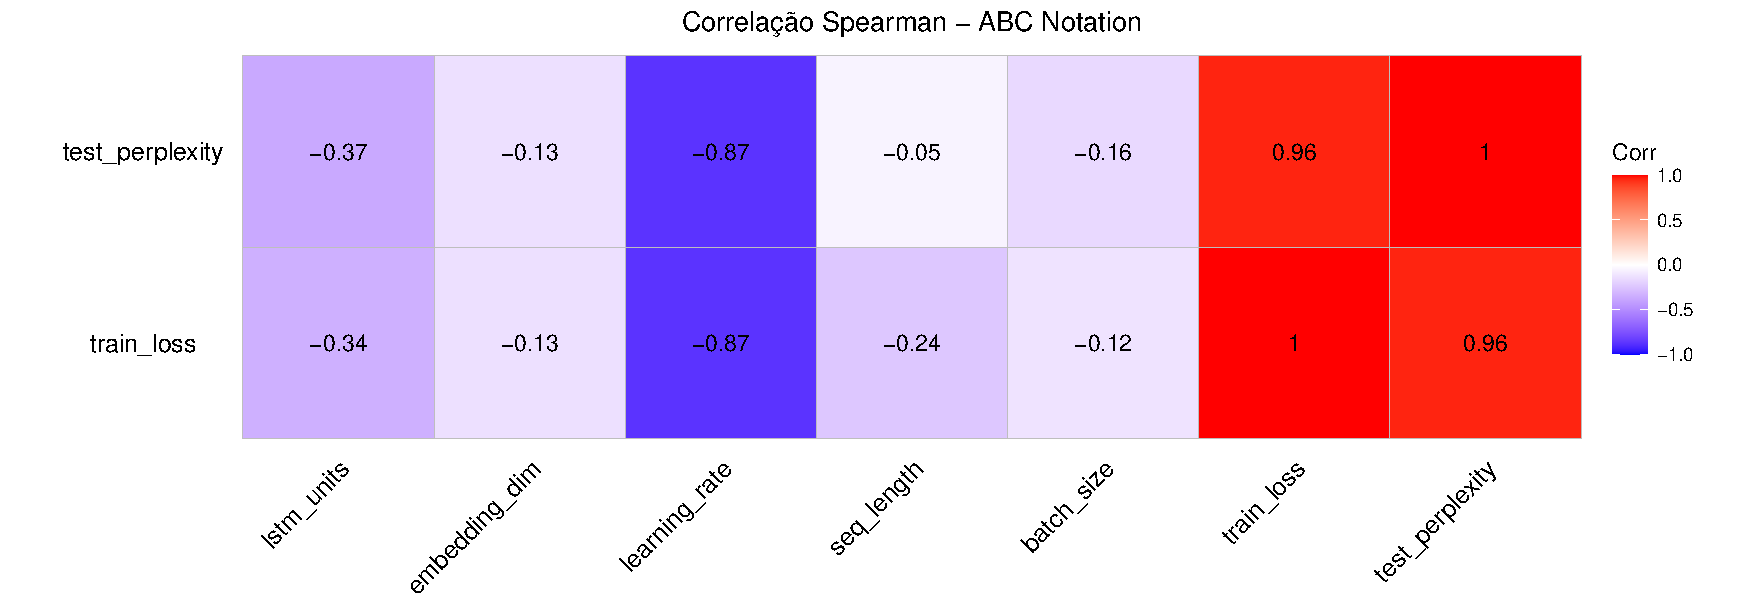
\includegraphics[width=\textwidth]{abcnotation_tanh_corr.pdf}
    \caption{Correlação entre parâmetros e métricas para ABC Notation}
    \label{fig:abcnotation_tanh_corr}
\end{figure}

\rowcolors{2}{gray!25}{white}
\begin{table}[H]
    \caption{Resultados dos experimentos referentes à base de dados ABC Notation, com $vocab\_size = 125$, utilizando a função \textit{tanh} como função de ativação. Em azul
(vermelho), constam os dois melhores (piores) modelos em relação à perplexidade.} \label{table:abcnotation_tanh_full}
    \centering
    \resizebox{\linewidth}{!}{
        \begin{tabular}[t]{ccccccccc}
        \toprule
        idx & lstm\_units & embedding\_dim & learning\_rate & seq\_length & batch\_size & train\_loss & test\_perplexity \\
        \midrule
        1 & 256 & 256 & $10^{-3}$ & 50 & 4 & 2.058 & 6.572 \\
        2 & 256 & 256 & $10^{-3}$ & 50 & 16 & 1.914 & 5.411 \\
        3 & 256 & 256 & $10^{-3}$ & 200 & 4 & 1.731 & 5.763 \\
        4 & 256 & 256 & $10^{-3}$ & 200 & 16 & 1.657 & 5.139 \\
        5 & 256 & 256 & $10^{-5}$ & 50 & 4 & 3.517 & 29.208 \\
        
        \red{6} & \red{256} & \red{256} & \red{$10^{-5}$} & \red{50} & \red{16} & \red{3.628} & \red{31.707} \\
        
        7 & 256 & 256 & $10^{-5}$ & 200 & 4 & 3.508 & 31.001 \\
        
        \red{8} & \red{256} & \red{256} & \red{$10^{-5}$} & \red{200} & \red{16} & \red{3.522} & \red{35.991} \\
        
        9 & 256 & 512 & $10^{-3}$ & 50 & 4 & 1.924 & 5.949 \\
        10 & 256 & 512 & $10^{-3}$ & 50 & 16 & 1.877 & 5.255 \\
        11 & 256 & 512 & $10^{-3}$ & 200 & 4 & 1.675 & 5.505 \\
        12 & 256 & 512 & $10^{-3}$ & 200 & 16 & 1.587 & 4.870 \\
        13 & 256 & 512 & $10^{-5}$ & 50 & 4 & 3.483 & 28.005 \\
        14 & 256 & 512 & $10^{-5}$ & 50 & 16 & 3.517 & 28.052 \\
        15 & 256 & 512 & $10^{-5}$ & 200 & 4 & 3.435 & 29.033 \\
        16 & 256 & 512 & $10^{-5}$ & 200 & 16 & 3.369 & 30.867 \\
        17 & 1024 & 256 & $10^{-3}$ & 50 & 4 & 1.782 & 5.690 \\
        18 & 1024 & 256 & $10^{-3}$ & 50 & 16 & 1.660 & 4.268 \\
        19 & 1024 & 256 & $10^{-3}$ & 200 & 4 & 1.487 & 4.507 \\
        
        \blue{20} & \blue{1024} & \blue{256} & \blue{$10^{-3}$} & \blue{200} & \blue{16} & \blue{1.350} & \blue{3.971} \\
        
        21 & 1024 & 256 & $10^{-5}$ & 50 & 4 & 3.452 & 27.038 \\
        22 & 1024 & 256 & $10^{-5}$ & 50 & 16 & 3.350 & 22.821 \\
        23 & 1024 & 256 & $10^{-5}$ & 200 & 4 & 3.387 & 26.320 \\
        24 & 1024 & 256 & $10^{-5}$ & 200 & 16 & 3.156 & 26.029 \\
        25 & 1024 & 512 & $10^{-3}$ & 50 & 4 & 1.767 & 5.611 \\
        26 & 1024 & 512 & $10^{-3}$ & 50 & 16 & 1.635 & 4.274 \\
        27 & 1024 & 512 & $10^{-3}$ & 200 & 4 & 1.361 & 4.342 \\
        
        \blue{28} & \blue{1024} & \blue{512} & \blue{$10^{-3}$} & \blue{200} & \blue{16} & \blue{1.305} & \blue{3.940} \\
        
        29 & 1024 & 512 & $10^{-5}$ & 50 & 4 & 3.366 & 22.080 \\
        30 & 1024 & 512 & $10^{-5}$ & 50 & 16 & 3.148 & 19.285 \\
        31 & 1024 & 512 & $10^{-5}$ & 200 & 4 & 3.210 & 22.511 \\
        32 & 1024 & 512 & $10^{-5}$ & 200 & 16 & 2.968 & 22.439 \\
        \bottomrule
        \end{tabular}
    }
\end{table}

\rowcolors{3}{white}{gray!25}
\begin{table}[H]
    \label{tab:abcnotation_tanh_vs_logit}
    \caption{ABC Notation: \textit{tanh} vs \textit{logit}}
    \centering
    \begin{tabular}{c|cc|cc}
        \toprule
        \multirow{2}{*}{idx} &
        \multicolumn{2}{c}{\textit{train\_loss}} &
        \multicolumn{2}{c}{\textit{test\_perplexity}} \\
        & {\textit{tanh}} & {\textit{logit}} & {\textit{tanh}} & {\textit{logit}} \\
        \midrule
        8 & 3.628 & 3.670 & 31.707 & 33.038 \\
        6 & 3.522 & 3.571 & 35.991 & 37.849 \\
        20 & 1.350 & 1.616 & 3.971 & 5.142 \\
        28 & 1.305 & 1.585 & 3.940 & 4.960 \\
    \bottomrule
  \end{tabular}
\end{table}

Também, na figura \ref{fig:abcnotation_tanh_vs_logit} são comparadas as curvas de perda dos modelos com cada função de ativação. Observou-se que o ajuste dos modelos com \textit{logit} apresentou um comportamento mais suave nos modelos $idx \in \{8,6\}$, não ocorrendo a mesma queda abrupta próxima da época 250 observada na \textit{tanh}. Por fim, pode-se concluir que a função \textit{tanh} apresentou melhores resultados para a base ABC Notation. Nessa etapa, os resultados são similares aos vistos na base de dados Irish. 

\begin{figure}
    \centering
    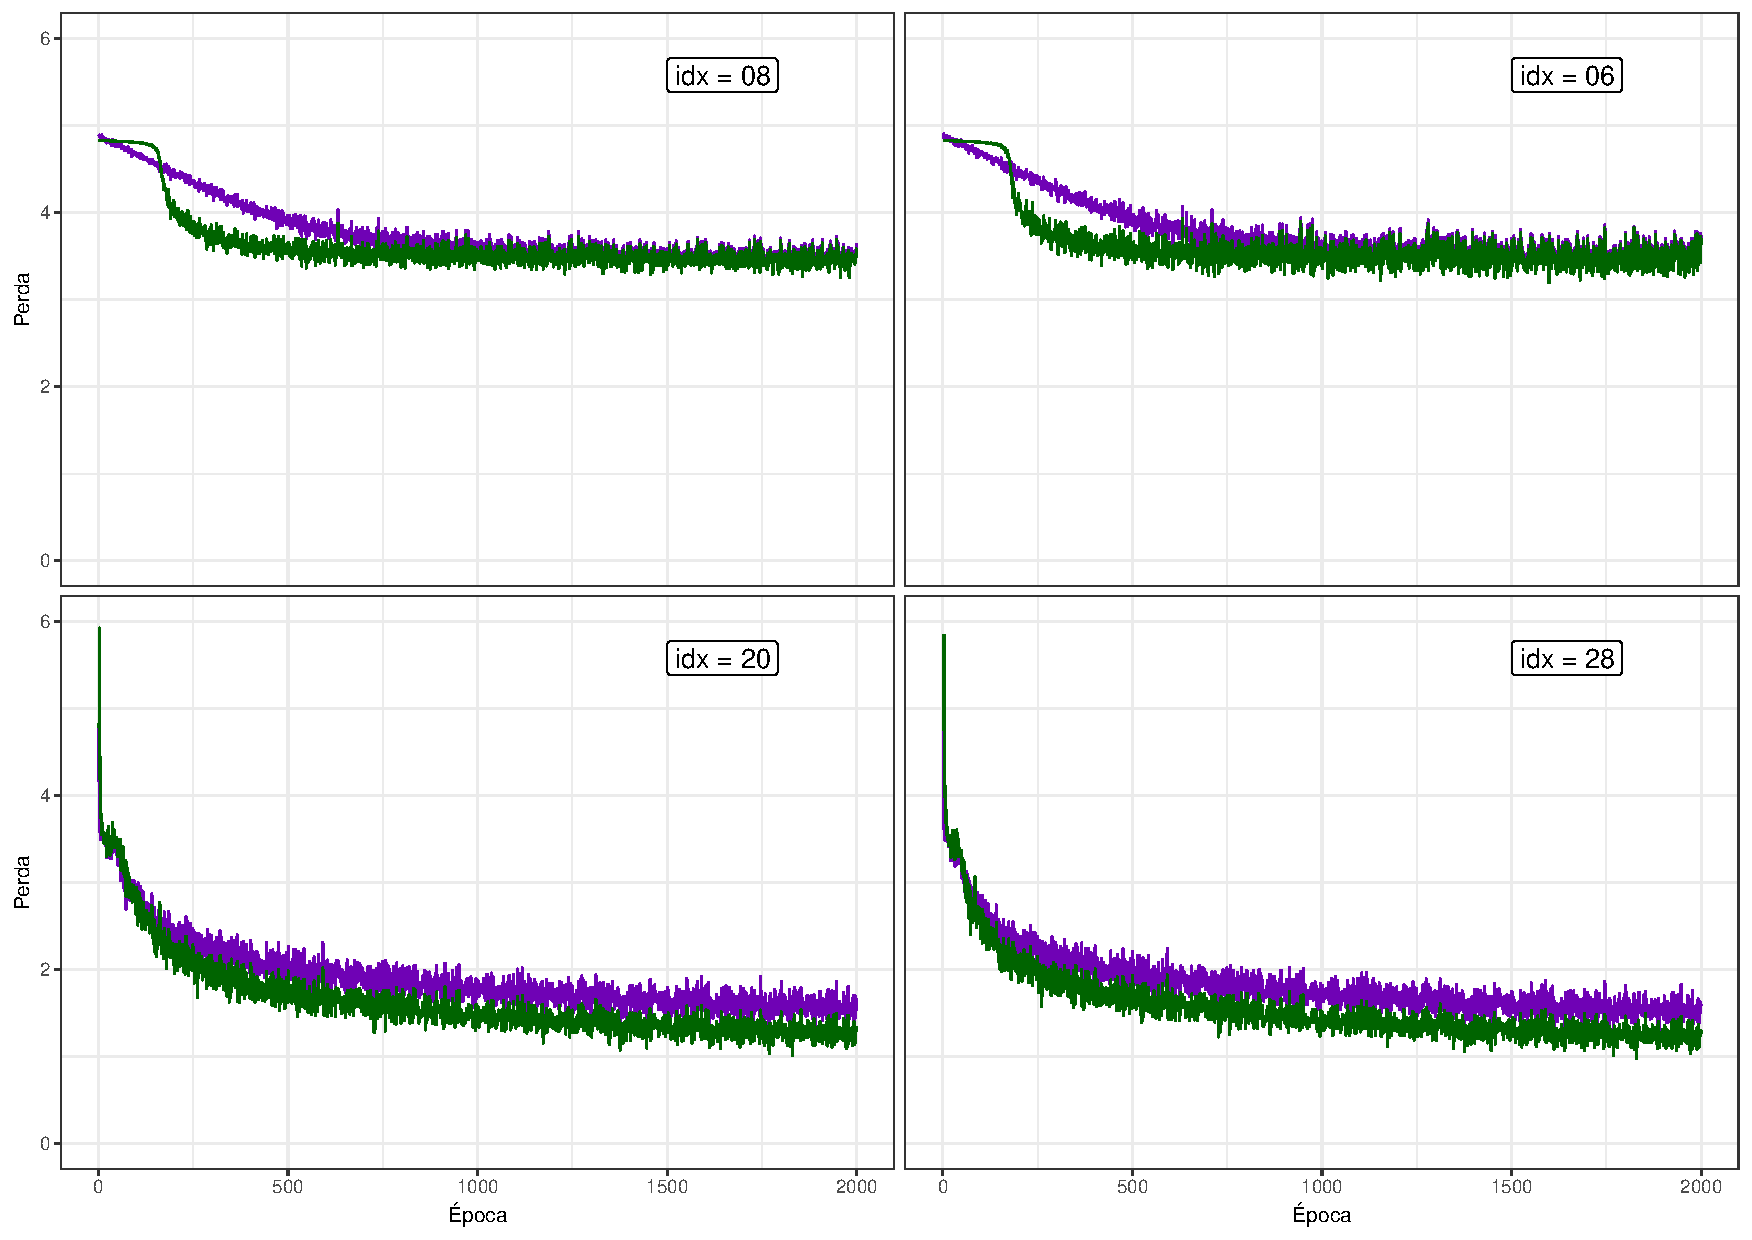
\includegraphics[width=\textwidth]{abcnotation_tanh_vs_logit.pdf}
    \caption{ABC Notation: \textit{tanh} (verde) vs \textit{logit} (roxo)}
    \label{fig:abcnotation_tanh_vs_logit}
\end{figure}



    % Músicas Geradas
\section{Músicas Geradas}
Para cada modelo selecionado na segunda etapa, considerando ambas as bases e ambas as funções de ativação, foram geradas sequências de texto até compor dez blocos candidatos a músicas. Após isso, realizou-se a conversão dos arquivos \textit{.abc} em música. Se a conversão é bem sucedida, uma nova peça musical é gerada; caso contrário, o arquivo é invalidado. Por não ter sido imposta uma estrutura que garanta a conversão, nem todo \textit{.abc} resultante gera uma música. Os resultados observados seguem:
\begin{itemize}
    \item Apenas candidatos dos melhores modelos foram convertidos com sucesso (porém não todos). Isso indica que uma menor perplexidade contribui para que o texto produzido seja mais coerente para a conversão em música.
    \item Há uma maior taxa de conversão nos modelos utilizando \textit{tanh} do que \textit{logit}, sendo mais um indicativo de que a primeira apresenta desempenho superior à segunda.
\end{itemize}
Em síntese, foram geradas 24 músicas com Irish ($10$ para $idx=11$ - com $6$ para \textit{tanh} e $4$ para \textit{logit} - e $14$ para $idx=25$ - com $8$ para \textit{tanh} e $6$ para \textit{logit}) e 14 com ABC Notation ($8$ para $idx=20$ - $4$ para cada função de ativação - e $6$ para $idx=28$ - com $5$ para \textit{tanh} e $1$ para \textit{logit}).

Ao escutarmos as músicas geradas para Irish, observa-se um certo padrão: diversos trechos são, via de regra, similares. É possível que o fator que justifique esteja relacionado com uma característica das músicas utilizadas no ajuste da rede neural. Além disso, é curioso observar que um dos arquivos \textit{.abc} convertidos não tem, na realidade, nenhuma nota musical. Ou seja, foi criada a estrutura do arquivo sem nenhum preenchimento referente a música. Por fim, pode-se concluir que as peças musicais resultantes são musicalmente plausíveis.

No caso das músicas geradas com ABC Notation, o comportamento é mais interessante. Inicialmente, é clara a maior variabilidade utilizando essa base, sendo identificado estilos e até mesmos duas vozes sendo executadas simultaneamente (como mão direita e mão esquerda do piano). Ademais, uma das peças musicais geradas destoou das demais, apresentando combinações de notas aparentemente mais ruidosas. Novamente, surgiram arquivos convertidos sem música. Por conseguinte, temos, mais uma vez, resultados musicalmente plausíveis.

Os comentários feitos referente às composições geradas são as percepções do autor com seu limitado conhecimento musical. Para o leitor interessado, todo o material produzido para este trabalho está disponível conforme informado na seção \ref{computacional}, incluindo as músicas.




%%%%%%%%%%%%%%%%%%%%%%%%%%%%%%%%%%%
%%%%  Conclusão e Trabalhos Futuros
%%%%%%%%%%%%%%%%%%%%%%%%%%%%%%%%%%%
\chapter{Considerações Finais}

%\pumi{Sugiro recapitular o que foi feito no trabalho em um pequeno parágrafo. }
%\nico{Interpreto o primeiro parágrafo como um certo ``resumo''}

%Este trabalho visou a explorar o problema de composição automática de músicas. Via modificações dos parâmetros do modelo utilizado, foram identificados padrões referentes à modelagem que, em suma, não são muito investigados. Ainda, observou-se que valores menores de perplexidade contribuem para a etapa de geração musical, posto que não houve nenhuma peça musical produzida pelas redes com altos valores na métrica.

Este trabalho visou a explorar o problema de composição automática de músicas. Via modificações dos parâmetros, investigou-se a sensibilidade do modelo utilizado para a geração de arquivos \textit{.abc} que, posteriormente, foram convertidos em novas peças musicais. Com o auxílio da medida perplexidade, foi possível mensurar se houveram (ou não) mudanças nos resultados de cada configuração da rede neural. Também, observou-se que a função de ativação \textit{tanh} teve desempenho superior na métrica para os cenários testados. Por fim, pode-se concluir que valores menores de perplexidade contribuem para a etapa de geração musical, posto que não houve nenhuma peça produzida pelas redes com resultados altos na métrica. 

Considerando a natureza subjetiva da música, o autor comentou sobre suas próprias percepções referente às composições. Devido a isso, os pontos elencados podem conflitar com outros pontos de vista. Isso posto, observou-se um padrão nas peças musicais produzidas pela rede ajustada com Irish, sendo bastante similares em perfil de ritmo e sequência de notas musicais. No caso de ABC Notation, houve uma maior variabilidade de estilos em comparação, além do fato de ter surgido uma peça aparentemente mais ruidosa. De maneira sucinta, conclui-se que os resultados são musicalmente plausíveis.

É importante destacar que há muito a ser investigado no problema de composição algorítmica utilizando inteligência artificial. O presente trabalho concentrou-se em apenas um único modelo com uma única arquitetura. Assim sendo, extensões envolvem modificar a arquitetura contemplando o aumento do número de camadas, tal como outros perfis de redes, como a \textit{transformer} \citep{vaswani2017}. No contexto das composições, analisar detalhadamente características musicais almejando, talvez, peças com estilos específicos.



%%%%%%%%%%%%%%%%%%%%%%%%%%%%%%%%%%%
%%%%  Referências
%%%%%%%%%%%%%%%%%%%%%%%%%%%%%%%%%%%
\addcontentsline{toc}{chapter}{Referências Bibliográficas} % Coloca no sumário
\bibliographystyle{apalike-br}
\bibliography{biblio}


%\printindex % Opcional  Índice remissivo

\end{document}
